\documentclass[11pt]{article}
\usepackage[margin=1in]{geometry}
\usepackage[T1]{fontenc}
\usepackage{lmodern}
\usepackage{amsmath,amssymb,booktabs,icomma,array,graphicx,tabularx}
\usepackage[round]{natbib}
\usepackage{placeins}
% refs.bib notes contain literal underscores (file names, DOIs).
\usepackage[strings]{underscore}
\usepackage[hidelinks]{hyperref}

% Result numbers. Generated by `crew.py numbers`; never typed by hand.
% Generated by `crew.py numbers` from claims.jsonl. Do not edit by hand.
% Each macro is a number taken from a logged run; see claims.jsonl.
\newcommand{\NoctrlCoef}{19,559}  % noctrl-coef
\newcommand{\NoctrlSeHC}{1,413}  % noctrl-se-hc0
\newcommand{\NoctrlSeClassical}{1,306}  % noctrl-se-classical
\newcommand{\NoctrlN}{9,915}  % noctrl-n
\newcommand{\NoctrlDiff}{0.34}  % noctrl-diff
\newcommand{\NoctrlBandCoef}{18,858}  % noctrl-band-coef
\newcommand{\NoctrlBandN}{9,275}  % noctrl-band-n
\newcommand{\ThetaLassoTwo}{7,701}  % plr-lasso-2fold
\newcommand{\PubThetaLassoTwo}{7,717}  % plr-lasso-2fold-pub
\newcommand{\PubSeMedLassoTwo}{1,346}  % plr-lasso-2fold-pub-se-med
\newcommand{\PubSeAdjLassoTwo}{1,749}  % plr-lasso-2fold-pub-se-adj
\newcommand{\SeMedLassoTwo}{1,345}  % plr-lasso-2fold-se-med
\newcommand{\SeAdjLassoTwo}{1,377}  % plr-lasso-2fold-se-adj
\newcommand{\CiLowLassoTwo}{5,002}  % plr-lasso-2fold-ci-low
\newcommand{\DiffLassoTwo}{-16}  % plr-lasso-2fold-diff
\newcommand{\DiffPubSeLassoTwo}{-0.01}  % plr-lasso-2fold-diff-pubse
\newcommand{\TolLassoTwo}{825}  % plr-lasso-2fold-tol
\newcommand{\MdsLassoTwo}{1,072}  % plr-lasso-2fold-mds
\newcommand{\TolObsLassoTwo}{596}  % plr-lasso-2fold-tol-obs
\newcommand{\PctIneligLassoTwo}{71}  % plr-lasso-2fold-pct-inelig
\newcommand{\PubPctIneligLassoTwo}{72}  % plr-lasso-2fold-pub-pct-inelig
\newcommand{\SdUnitsLassoTwo}{0.121}  % plr-lasso-2fold-sd-units
\newcommand{\PubSdUnitsLassoTwo}{0.121}  % plr-lasso-2fold-pub-sd-units
\newcommand{\SplitSdObsLassoTwo}{354}  % plr-lasso-2fold-split-sd-obs
\newcommand{\SplitSdPubLassoTwo}{1,656}  % plr-lasso-2fold-split-sd-pub
\newcommand{\ImpliedMadObsLassoTwo}{295}  % plr-lasso-2fold-implied-mad-obs
\newcommand{\ImpliedMadPubLassoTwo}{1,117}  % plr-lasso-2fold-implied-mad-pub
\newcommand{\SeMedRatioLassoTwo}{1.00}  % plr-lasso-2fold-se-med-ratio
\newcommand{\SeAdjRatioLassoTwo}{0.79}  % plr-lasso-2fold-se-adj-ratio
\newcommand{\RmseLLassoTwo}{54,872}  % plr-lasso-2fold-rmse-l
\newcommand{\RmseMLassoTwo}{0.4486}  % plr-lasso-2fold-rmse-m
\newcommand{\MOutLassoTwo}{0.0000}  % plr-lasso-2fold-m-out
\newcommand{\ThetaMinLassoTwo}{6,826}  % plr-lasso-2fold-theta-min
\newcommand{\ThetaMaxLassoTwo}{8,675}  % plr-lasso-2fold-theta-max
\newcommand{\ThetaLassoFive}{8,173}  % plr-lasso-5fold
\newcommand{\PubThetaLassoFive}{8,187}  % plr-lasso-5fold-pub
\newcommand{\PubSeMedLassoFive}{1,298}  % plr-lasso-5fold-pub-se-med
\newcommand{\PubSeAdjLassoFive}{1,558}  % plr-lasso-5fold-pub-se-adj
\newcommand{\SeMedLassoFive}{1,300}  % plr-lasso-5fold-se-med
\newcommand{\SeAdjLassoFive}{1,309}  % plr-lasso-5fold-se-adj
\newcommand{\CiLowLassoFive}{5,607}  % plr-lasso-5fold-ci-low
\newcommand{\DiffLassoFive}{-14}  % plr-lasso-5fold-diff
\newcommand{\DiffPubSeLassoFive}{-0.01}  % plr-lasso-5fold-diff-pubse
\newcommand{\TolLassoFive}{636}  % plr-lasso-5fold-tol
\newcommand{\MdsLassoFive}{827}  % plr-lasso-5fold-mds
\newcommand{\TolObsLassoFive}{455}  % plr-lasso-5fold-tol-obs
\newcommand{\PctIneligLassoFive}{76}  % plr-lasso-5fold-pct-inelig
\newcommand{\PubPctIneligLassoFive}{76}  % plr-lasso-5fold-pub-pct-inelig
\newcommand{\SdUnitsLassoFive}{0.129}  % plr-lasso-5fold-sd-units
\newcommand{\PubSdUnitsLassoFive}{0.129}  % plr-lasso-5fold-pub-sd-units
\newcommand{\SplitSdObsLassoFive}{190}  % plr-lasso-5fold-split-sd-obs
\newcommand{\SplitSdPubLassoFive}{1,278}  % plr-lasso-5fold-split-sd-pub
\newcommand{\ImpliedMadObsLassoFive}{152}  % plr-lasso-5fold-implied-mad-obs
\newcommand{\ImpliedMadPubLassoFive}{862}  % plr-lasso-5fold-implied-mad-pub
\newcommand{\SeMedRatioLassoFive}{1.00}  % plr-lasso-5fold-se-med-ratio
\newcommand{\SeAdjRatioLassoFive}{0.84}  % plr-lasso-5fold-se-adj-ratio
\newcommand{\RmseLLassoFive}{54,560}  % plr-lasso-5fold-rmse-l
\newcommand{\RmseMLassoFive}{0.4477}  % plr-lasso-5fold-rmse-m
\newcommand{\MOutLassoFive}{0.0000}  % plr-lasso-5fold-m-out
\newcommand{\ThetaMinLassoFive}{7,590}  % plr-lasso-5fold-theta-min
\newcommand{\ThetaMaxLassoFive}{8,546}  % plr-lasso-5fold-theta-max
\newcommand{\ThetaTreeTwo}{8,767}  % plr-tree-2fold
\newcommand{\PubThetaTreeTwo}{8,709}  % plr-tree-2fold-pub
\newcommand{\PubSeMedTreeTwo}{1,363}  % plr-tree-2fold-pub-se-med
\newcommand{\PubSeAdjTreeTwo}{1,427}  % plr-tree-2fold-pub-se-adj
\newcommand{\SeMedTreeTwo}{1,355}  % plr-tree-2fold-se-med
\newcommand{\SeAdjTreeTwo}{1,413}  % plr-tree-2fold-se-adj
\newcommand{\CiLowTreeTwo}{5,997}  % plr-tree-2fold-ci-low
\newcommand{\DiffTreeTwo}{58}  % plr-tree-2fold-diff
\newcommand{\DiffPubSeTreeTwo}{0.04}  % plr-tree-2fold-diff-pubse
\newcommand{\TolTreeTwo}{312}  % plr-tree-2fold-tol
\newcommand{\MdsTreeTwo}{405}  % plr-tree-2fold-mds
\newcommand{\TolObsTreeTwo}{291}  % plr-tree-2fold-tol-obs
\newcommand{\PctIneligTreeTwo}{81}  % plr-tree-2fold-pct-inelig
\newcommand{\PubPctIneligTreeTwo}{81}  % plr-tree-2fold-pub-pct-inelig
\newcommand{\SdUnitsTreeTwo}{0.138}  % plr-tree-2fold-sd-units
\newcommand{\PubSdUnitsTreeTwo}{0.137}  % plr-tree-2fold-pub-sd-units
\newcommand{\SplitSdObsTreeTwo}{541}  % plr-tree-2fold-split-sd-obs
\newcommand{\SplitSdPubTreeTwo}{626}  % plr-tree-2fold-split-sd-pub
\newcommand{\ImpliedMadObsTreeTwo}{403}  % plr-tree-2fold-implied-mad-obs
\newcommand{\ImpliedMadPubTreeTwo}{423}  % plr-tree-2fold-implied-mad-pub
\newcommand{\SeMedRatioTreeTwo}{0.99}  % plr-tree-2fold-se-med-ratio
\newcommand{\SeAdjRatioTreeTwo}{0.99}  % plr-tree-2fold-se-adj-ratio
\newcommand{\RmseLTreeTwo}{57,209}  % plr-tree-2fold-rmse-l
\newcommand{\RmseMTreeTwo}{0.4497}  % plr-tree-2fold-rmse-m
\newcommand{\MOutTreeTwo}{0.0000}  % plr-tree-2fold-m-out
\newcommand{\ThetaMinTreeTwo}{7,395}  % plr-tree-2fold-theta-min
\newcommand{\ThetaMaxTreeTwo}{10,184}  % plr-tree-2fold-theta-max
\newcommand{\ThetaTreeFive}{8,934}  % plr-tree-5fold
\newcommand{\PubThetaTreeFive}{8,871}  % plr-tree-5fold-pub
\newcommand{\PubSeMedTreeFive}{1,358}  % plr-tree-5fold-pub-se-med
\newcommand{\PubSeAdjTreeFive}{1,418}  % plr-tree-5fold-pub-se-adj
\newcommand{\SeMedTreeFive}{1,353}  % plr-tree-5fold-se-med
\newcommand{\SeAdjTreeFive}{1,375}  % plr-tree-5fold-se-adj
\newcommand{\CiLowTreeFive}{6,240}  % plr-tree-5fold-ci-low
\newcommand{\DiffTreeFive}{63}  % plr-tree-5fold-diff
\newcommand{\DiffPubSeTreeFive}{0.05}  % plr-tree-5fold-diff-pubse
\newcommand{\TolTreeFive}{301}  % plr-tree-5fold-tol
\newcommand{\MdsTreeFive}{392}  % plr-tree-5fold-mds
\newcommand{\TolObsTreeFive}{247}  % plr-tree-5fold-tol-obs
\newcommand{\PctIneligTreeFive}{83}  % plr-tree-5fold-pct-inelig
\newcommand{\PubPctIneligTreeFive}{82}  % plr-tree-5fold-pub-pct-inelig
\newcommand{\SdUnitsTreeFive}{0.141}  % plr-tree-5fold-sd-units
\newcommand{\PubSdUnitsTreeFive}{0.140}  % plr-tree-5fold-pub-sd-units
\newcommand{\SplitSdObsTreeFive}{354}  % plr-tree-5fold-split-sd-obs
\newcommand{\SplitSdPubTreeFive}{605}  % plr-tree-5fold-split-sd-pub
\newcommand{\ImpliedMadObsTreeFive}{243}  % plr-tree-5fold-implied-mad-obs
\newcommand{\ImpliedMadPubTreeFive}{408}  % plr-tree-5fold-implied-mad-pub
\newcommand{\SeMedRatioTreeFive}{1.00}  % plr-tree-5fold-se-med-ratio
\newcommand{\SeAdjRatioTreeFive}{0.97}  % plr-tree-5fold-se-adj-ratio
\newcommand{\RmseLTreeFive}{57,183}  % plr-tree-5fold-rmse-l
\newcommand{\RmseMTreeFive}{0.4501}  % plr-tree-5fold-rmse-m
\newcommand{\MOutTreeFive}{0.0000}  % plr-tree-5fold-m-out
\newcommand{\ThetaMinTreeFive}{8,115}  % plr-tree-5fold-theta-min
\newcommand{\ThetaMaxTreeFive}{9,906}  % plr-tree-5fold-theta-max
\newcommand{\ThetaForestTwo}{9,064}  % plr-forest-2fold
\newcommand{\PubThetaForestTwo}{9,116}  % plr-forest-2fold-pub
\newcommand{\PubSeMedForestTwo}{1,302}  % plr-forest-2fold-pub-se-med
\newcommand{\PubSeAdjForestTwo}{1,377}  % plr-forest-2fold-pub-se-adj
\newcommand{\SeMedForestTwo}{1,255}  % plr-forest-2fold-se-med
\newcommand{\SeAdjForestTwo}{1,319}  % plr-forest-2fold-se-adj
\newcommand{\CiLowForestTwo}{6,479}  % plr-forest-2fold-ci-low
\newcommand{\DiffForestTwo}{-52}  % plr-forest-2fold-diff
\newcommand{\DiffPubSeForestTwo}{-0.04}  % plr-forest-2fold-diff-pubse
\newcommand{\TolForestTwo}{438}  % plr-forest-2fold-tol
\newcommand{\MdsForestTwo}{569}  % plr-forest-2fold-mds
\newcommand{\TolObsForestTwo}{396}  % plr-forest-2fold-tol-obs
\newcommand{\PctIneligForestTwo}{84}  % plr-forest-2fold-pct-inelig
\newcommand{\PubPctIneligForestTwo}{85}  % plr-forest-2fold-pub-pct-inelig
\newcommand{\SdUnitsForestTwo}{0.143}  % plr-forest-2fold-sd-units
\newcommand{\PubSdUnitsForestTwo}{0.144}  % plr-forest-2fold-pub-sd-units
\newcommand{\SplitSdObsForestTwo}{574}  % plr-forest-2fold-split-sd-obs
\newcommand{\SplitSdPubForestTwo}{665}  % plr-forest-2fold-split-sd-pub
\newcommand{\ImpliedMadObsForestTwo}{405}  % plr-forest-2fold-implied-mad-obs
\newcommand{\ImpliedMadPubForestTwo}{448}  % plr-forest-2fold-implied-mad-pub
\newcommand{\SeMedRatioForestTwo}{0.96}  % plr-forest-2fold-se-med-ratio
\newcommand{\SeAdjRatioForestTwo}{0.96}  % plr-forest-2fold-se-adj-ratio
\newcommand{\RmseLForestTwo}{54,976}  % plr-forest-2fold-rmse-l
\newcommand{\RmseMForestTwo}{0.4622}  % plr-forest-2fold-rmse-m
\newcommand{\MOutForestTwo}{0.0146}  % plr-forest-2fold-m-out
\newcommand{\ThetaMinForestTwo}{7,889}  % plr-forest-2fold-theta-min
\newcommand{\ThetaMaxForestTwo}{9,786}  % plr-forest-2fold-theta-max
\newcommand{\ThetaForestFive}{9,041}  % plr-forest-5fold
\newcommand{\PubThetaForestFive}{9,247}  % plr-forest-5fold-pub
\newcommand{\PubSeMedForestFive}{1,295}  % plr-forest-5fold-pub-se-med
\newcommand{\PubSeAdjForestFive}{1,328}  % plr-forest-5fold-pub-se-adj
\newcommand{\SeMedForestFive}{1,230}  % plr-forest-5fold-se-med
\newcommand{\SeAdjForestFive}{1,259}  % plr-forest-5fold-se-adj
\newcommand{\CiLowForestFive}{6,573}  % plr-forest-5fold-ci-low
\newcommand{\DiffForestFive}{-206}  % plr-forest-5fold-diff
\newcommand{\DiffPubSeForestFive}{-0.16}  % plr-forest-5fold-diff-pubse
\newcommand{\TolForestFive}{287}  % plr-forest-5fold-tol
\newcommand{\MdsForestFive}{373}  % plr-forest-5fold-mds
\newcommand{\TolObsForestFive}{239}  % plr-forest-5fold-tol-obs
\newcommand{\PctIneligForestFive}{84}  % plr-forest-5fold-pct-inelig
\newcommand{\PubPctIneligForestFive}{86}  % plr-forest-5fold-pub-pct-inelig
\newcommand{\SdUnitsForestFive}{0.142}  % plr-forest-5fold-sd-units
\newcommand{\PubSdUnitsForestFive}{0.146}  % plr-forest-5fold-pub-sd-units
\newcommand{\SplitSdObsForestFive}{328}  % plr-forest-5fold-split-sd-obs
\newcommand{\SplitSdPubForestFive}{436}  % plr-forest-5fold-split-sd-pub
\newcommand{\ImpliedMadObsForestFive}{269}  % plr-forest-5fold-implied-mad-obs
\newcommand{\ImpliedMadPubForestFive}{294}  % plr-forest-5fold-implied-mad-pub
\newcommand{\SeMedRatioForestFive}{0.95}  % plr-forest-5fold-se-med-ratio
\newcommand{\SeAdjRatioForestFive}{0.95}  % plr-forest-5fold-se-adj-ratio
\newcommand{\RmseLForestFive}{54,678}  % plr-forest-5fold-rmse-l
\newcommand{\RmseMForestFive}{0.4627}  % plr-forest-5fold-rmse-m
\newcommand{\MOutForestFive}{0.0157}  % plr-forest-5fold-m-out
\newcommand{\ThetaMinForestFive}{8,347}  % plr-forest-5fold-theta-min
\newcommand{\ThetaMaxForestFive}{10,035}  % plr-forest-5fold-theta-max
\newcommand{\ThetaBoostingTwo}{8,830}  % plr-boosting-2fold
\newcommand{\PubThetaBoostingTwo}{8,759}  % plr-boosting-2fold-pub
\newcommand{\PubSeMedBoostingTwo}{1,339}  % plr-boosting-2fold-pub-se-med
\newcommand{\PubSeAdjBoostingTwo}{1,382}  % plr-boosting-2fold-pub-se-adj
\newcommand{\SeMedBoostingTwo}{1,336}  % plr-boosting-2fold-se-med
\newcommand{\SeAdjBoostingTwo}{1,363}  % plr-boosting-2fold-se-adj
\newcommand{\CiLowBoostingTwo}{6,159}  % plr-boosting-2fold-ci-low
\newcommand{\DiffBoostingTwo}{71}  % plr-boosting-2fold-diff
\newcommand{\DiffPubSeBoostingTwo}{0.05}  % plr-boosting-2fold-diff-pubse
\newcommand{\TolBoostingTwo}{372}  % plr-boosting-2fold-tol
\newcommand{\MdsBoostingTwo}{483}  % plr-boosting-2fold-mds
\newcommand{\TolObsBoostingTwo}{291}  % plr-boosting-2fold-tol-obs
\newcommand{\PctIneligBoostingTwo}{82}  % plr-boosting-2fold-pct-inelig
\newcommand{\PubPctIneligBoostingTwo}{81}  % plr-boosting-2fold-pub-pct-inelig
\newcommand{\SdUnitsBoostingTwo}{0.139}  % plr-boosting-2fold-sd-units
\newcommand{\PubSdUnitsBoostingTwo}{0.138}  % plr-boosting-2fold-pub-sd-units
\newcommand{\SplitSdObsBoostingTwo}{358}  % plr-boosting-2fold-split-sd-obs
\newcommand{\SplitSdPubBoostingTwo}{507}  % plr-boosting-2fold-split-sd-pub
\newcommand{\ImpliedMadObsBoostingTwo}{271}  % plr-boosting-2fold-implied-mad-obs
\newcommand{\ImpliedMadPubBoostingTwo}{342}  % plr-boosting-2fold-implied-mad-pub
\newcommand{\SeMedRatioBoostingTwo}{1.00}  % plr-boosting-2fold-se-med-ratio
\newcommand{\SeAdjRatioBoostingTwo}{0.99}  % plr-boosting-2fold-se-adj-ratio
\newcommand{\RmseLBoostingTwo}{55,112}  % plr-boosting-2fold-rmse-l
\newcommand{\RmseMBoostingTwo}{0.4435}  % plr-boosting-2fold-rmse-m
\newcommand{\MOutBoostingTwo}{0.0000}  % plr-boosting-2fold-m-out
\newcommand{\ThetaMinBoostingTwo}{7,909}  % plr-boosting-2fold-theta-min
\newcommand{\ThetaMaxBoostingTwo}{9,522}  % plr-boosting-2fold-theta-max
\newcommand{\ThetaBoostingFive}{9,020}  % plr-boosting-5fold
\newcommand{\PubThetaBoostingFive}{9,110}  % plr-boosting-5fold-pub
\newcommand{\PubSeMedBoostingFive}{1,314}  % plr-boosting-5fold-pub-se-med
\newcommand{\PubSeAdjBoostingFive}{1,328}  % plr-boosting-5fold-pub-se-adj
\newcommand{\SeMedBoostingFive}{1,315}  % plr-boosting-5fold-se-med
\newcommand{\SeAdjBoostingFive}{1,325}  % plr-boosting-5fold-se-adj
\newcommand{\CiLowBoostingFive}{6,423}  % plr-boosting-5fold-ci-low
\newcommand{\DiffBoostingFive}{-90}  % plr-boosting-5fold-diff
\newcommand{\DiffPubSeBoostingFive}{-0.07}  % plr-boosting-5fold-diff-pubse
\newcommand{\TolBoostingFive}{209}  % plr-boosting-5fold-tol
\newcommand{\MdsBoostingFive}{272}  % plr-boosting-5fold-mds
\newcommand{\TolObsBoostingFive}{159}  % plr-boosting-5fold-tol-obs
\newcommand{\PctIneligBoostingFive}{84}  % plr-boosting-5fold-pct-inelig
\newcommand{\PubPctIneligBoostingFive}{84}  % plr-boosting-5fold-pub-pct-inelig
\newcommand{\SdUnitsBoostingFive}{0.142}  % plr-boosting-5fold-sd-units
\newcommand{\PubSdUnitsBoostingFive}{0.143}  % plr-boosting-5fold-pub-sd-units
\newcommand{\SplitSdObsBoostingFive}{191}  % plr-boosting-5fold-split-sd-obs
\newcommand{\SplitSdPubBoostingFive}{285}  % plr-boosting-5fold-split-sd-pub
\newcommand{\ImpliedMadObsBoostingFive}{159}  % plr-boosting-5fold-implied-mad-obs
\newcommand{\ImpliedMadPubBoostingFive}{192}  % plr-boosting-5fold-implied-mad-pub
\newcommand{\SeMedRatioBoostingFive}{1.00}  % plr-boosting-5fold-se-med-ratio
\newcommand{\SeAdjRatioBoostingFive}{1.00}  % plr-boosting-5fold-se-adj-ratio
\newcommand{\RmseLBoostingFive}{54,289}  % plr-boosting-5fold-rmse-l
\newcommand{\RmseMBoostingFive}{0.4430}  % plr-boosting-5fold-rmse-m
\newcommand{\MOutBoostingFive}{0.0000}  % plr-boosting-5fold-m-out
\newcommand{\ThetaMinBoostingFive}{8,540}  % plr-boosting-5fold-theta-min
\newcommand{\ThetaMaxBoostingFive}{9,406}  % plr-boosting-5fold-theta-max
\newcommand{\ThetaNnetTwo}{9,107}  % plr-nnet-2fold
\newcommand{\PubThetaNnetTwo}{8,950}  % plr-nnet-2fold-pub
\newcommand{\PubSeMedNnetTwo}{1,335}  % plr-nnet-2fold-pub-se-med
\newcommand{\PubSeAdjNnetTwo}{1,408}  % plr-nnet-2fold-pub-se-adj
\newcommand{\SeMedNnetTwo}{1,387}  % plr-nnet-2fold-se-med
\newcommand{\SeAdjNnetTwo}{1,428}  % plr-nnet-2fold-se-adj
\newcommand{\CiLowNnetTwo}{6,309}  % plr-nnet-2fold-ci-low
\newcommand{\DiffNnetTwo}{157}  % plr-nnet-2fold-diff
\newcommand{\DiffPubSeNnetTwo}{0.12}  % plr-nnet-2fold-diff-pubse
\newcommand{\TolNnetTwo}{330}  % plr-nnet-2fold-tol
\newcommand{\MdsNnetTwo}{429}  % plr-nnet-2fold-mds
\newcommand{\TolObsNnetTwo}{285}  % plr-nnet-2fold-tol-obs
\newcommand{\PctIneligNnetTwo}{84}  % plr-nnet-2fold-pct-inelig
\newcommand{\PubPctIneligNnetTwo}{83}  % plr-nnet-2fold-pub-pct-inelig
\newcommand{\SdUnitsNnetTwo}{0.143}  % plr-nnet-2fold-sd-units
\newcommand{\PubSdUnitsNnetTwo}{0.141}  % plr-nnet-2fold-pub-sd-units
\newcommand{\SplitSdObsNnetTwo}{464}  % plr-nnet-2fold-split-sd-obs
\newcommand{\SplitSdPubNnetTwo}{663}  % plr-nnet-2fold-split-sd-pub
\newcommand{\ImpliedMadObsNnetTwo}{339}  % plr-nnet-2fold-implied-mad-obs
\newcommand{\ImpliedMadPubNnetTwo}{447}  % plr-nnet-2fold-implied-mad-pub
\newcommand{\SeMedRatioNnetTwo}{1.04}  % plr-nnet-2fold-se-med-ratio
\newcommand{\SeAdjRatioNnetTwo}{1.01}  % plr-nnet-2fold-se-adj-ratio
\newcommand{\RmseLNnetTwo}{55,914}  % plr-nnet-2fold-rmse-l
\newcommand{\RmseMNnetTwo}{0.4462}  % plr-nnet-2fold-rmse-m
\newcommand{\MOutNnetTwo}{0.0231}  % plr-nnet-2fold-m-out
\newcommand{\ThetaMinNnetTwo}{7,236}  % plr-nnet-2fold-theta-min
\newcommand{\ThetaMaxNnetTwo}{10,350}  % plr-nnet-2fold-theta-max
\newcommand{\ThetaNnetFive}{9,126}  % plr-nnet-5fold
\newcommand{\PubThetaNnetFive}{9,038}  % plr-nnet-5fold-pub
\newcommand{\PubSeMedNnetFive}{1,322}  % plr-nnet-5fold-pub-se-med
\newcommand{\PubSeAdjNnetFive}{1,355}  % plr-nnet-5fold-pub-se-adj
\newcommand{\SeMedNnetFive}{1,383}  % plr-nnet-5fold-se-med
\newcommand{\SeAdjNnetFive}{1,408}  % plr-nnet-5fold-se-adj
\newcommand{\CiLowNnetFive}{6,366}  % plr-nnet-5fold-ci-low
\newcommand{\DiffNnetFive}{88}  % plr-nnet-5fold-diff
\newcommand{\DiffPubSeNnetFive}{0.07}  % plr-nnet-5fold-diff-pubse
\newcommand{\TolNnetFive}{219}  % plr-nnet-5fold-tol
\newcommand{\MdsNnetFive}{285}  % plr-nnet-5fold-mds
\newcommand{\TolObsNnetFive}{179}  % plr-nnet-5fold-tol-obs
\newcommand{\PctIneligNnetFive}{85}  % plr-nnet-5fold-pct-inelig
\newcommand{\PubPctIneligNnetFive}{84}  % plr-nnet-5fold-pub-pct-inelig
\newcommand{\SdUnitsNnetFive}{0.144}  % plr-nnet-5fold-sd-units
\newcommand{\PubSdUnitsNnetFive}{0.142}  % plr-nnet-5fold-pub-sd-units
\newcommand{\SplitSdObsNnetFive}{255}  % plr-nnet-5fold-split-sd-obs
\newcommand{\SplitSdPubNnetFive}{441}  % plr-nnet-5fold-split-sd-pub
\newcommand{\ImpliedMadObsNnetFive}{263}  % plr-nnet-5fold-implied-mad-obs
\newcommand{\ImpliedMadPubNnetFive}{297}  % plr-nnet-5fold-implied-mad-pub
\newcommand{\SeMedRatioNnetFive}{1.05}  % plr-nnet-5fold-se-med-ratio
\newcommand{\SeAdjRatioNnetFive}{1.04}  % plr-nnet-5fold-se-adj-ratio
\newcommand{\RmseLNnetFive}{55,932}  % plr-nnet-5fold-rmse-l
\newcommand{\RmseMNnetFive}{0.4442}  % plr-nnet-5fold-rmse-m
\newcommand{\MOutNnetFive}{0.0195}  % plr-nnet-5fold-m-out
\newcommand{\ThetaMinNnetFive}{8,177}  % plr-nnet-5fold-theta-min
\newcommand{\ThetaMaxNnetFive}{9,748}  % plr-nnet-5fold-theta-max
\newcommand{\HTwoNOutside}{0}  % h2-n-outside
\newcommand{\HTwoNTestableInside}{8}  % h2-n-testable-inside
\newcommand{\HTwoNTestable}{8}  % h2-n-testable
\newcommand{\HThreeMarginTwo}{1,066}  % h3-margin-k2
\newcommand{\HThreeMarginFive}{761}  % h3-margin-k5
\newcommand{\BaselineInelig}{10,788}  % baseline-inelig
\newcommand{\BaselineElig}{30,347}  % baseline-elig
\newcommand{\BaselineSd}{63,523}  % baseline-sd
\newcommand{\PortShiftLasso}{0.04}  % port-shift-lasso
\newcommand{\PortShiftSeLasso}{0.06}  % port-shift-se-lasso
\newcommand{\PortRmsLasso}{0.19}  % port-rms-lasso
\newcommand{\PortRmsSeedLasso}{0.00}  % port-rms-seed-lasso
\newcommand{\PortShiftTree}{-24.7}  % port-shift-tree
\newcommand{\PortShiftSeTree}{25.7}  % port-shift-se-tree
\newcommand{\PortRmsTree}{80.8}  % port-rms-tree
\newcommand{\PortRmsSeedTree}{83.9}  % port-rms-seed-tree
\newcommand{\PortShiftForest}{-216.0}  % port-shift-forest
\newcommand{\PortShiftSeForest}{9.4}  % port-shift-se-forest
\newcommand{\PortRmsForest}{217.9}  % port-rms-forest
\newcommand{\PortRmsSeedForest}{16.4}  % port-rms-seed-forest
\newcommand{\PortShiftBoosting}{-4.7}  % port-shift-boosting
\newcommand{\PortShiftSeBoosting}{2.6}  % port-shift-se-boosting
\newcommand{\PortRmsBoosting}{9.1}  % port-rms-boosting
\newcommand{\PortRmsSeedBoosting}{8.7}  % port-rms-seed-boosting
\newcommand{\PortShiftNnet}{-3.0}  % port-shift-nnet
\newcommand{\PortShiftSeNnet}{16.1}  % port-shift-se-nnet
\newcommand{\PortRmsNnet}{48.2}  % port-rms-nnet
\newcommand{\PortRmsSeedNnet}{33.6}  % port-rms-seed-nnet
\newcommand{\LassoCEffY}{0.5}  % lasso-c-eff-y
\newcommand{\LassoCEffD}{1.1}  % lasso-c-eff-d
\newcommand{\SensCElevenThetaTwo}{7,479}  % sens-c11-theta-k2
\newcommand{\SensCElevenSeAdjTwo}{1,434}  % sens-c11-se-adj-k2
\newcommand{\SensCElevenSeMedTwo}{1,406}  % sens-c11-se-med-k2
\newcommand{\SensCElevenDiffTwo}{-238}  % sens-c11-diff-k2
\newcommand{\SensCElevenMinusMainTwo}{-223}  % sens-c11-minus-main-k2
\newcommand{\SensCElevenHThreeMarginTwo}{1,289}  % sens-c11-h3-margin-k2
\newcommand{\SensCElevenThetaFive}{7,878}  % sens-c11-theta-k5
\newcommand{\SensCElevenSeAdjFive}{1,342}  % sens-c11-se-adj-k5
\newcommand{\SensCElevenSeMedFive}{1,333}  % sens-c11-se-med-k5
\newcommand{\SensCElevenDiffFive}{-309}  % sens-c11-diff-k5
\newcommand{\SensCElevenMinusMainFive}{-295}  % sens-c11-minus-main-k5
\newcommand{\SensCElevenHThreeMarginFive}{1,056}  % sens-c11-h3-margin-k5
\newcommand{\NnetIterY}{62}  % nnet-iter-y
\newcommand{\NnetIterD}{1000}  % nnet-iter-d


% Magnitude of a negative macro value (drops the leading minus sign of the macro's text).
\def\absvalaux-#1\relax{#1}
\newcommand{\absval}[1]{\expandafter\absvalaux#1\relax}
% A negative dollar amount from a macro, printed as -$x.
\newcommand{\negusd}[1]{$-$\$\absval{#1}}

\setlength{\emergencystretch}{2em}
\setlength{\belowcaptionskip}{6pt}
\renewcommand{\topfraction}{0.9}
\renewcommand{\bottomfraction}{0.8}
\renewcommand{\textfraction}{0.07}
\renewcommand{\floatpagefraction}{0.8}
\newcommand{\var}[1]{\texttt{#1}}
\newcolumntype{L}{>{\raggedright\arraybackslash}X}

\title{A Cell-by-Cell Check of the Double Machine Learning\\
401(k) Estimates of Chernozhukov et al.\ (2018)}
\author{Bryce Wang (human PI) \\ \small Drafted with Free-Research-Crew; see the AI-use statement.}
\date{\today}

\begin{document}
\maketitle

\begin{abstract}
\noindent
We re-estimate the ten partially linear double machine learning (DML) estimates of
\citet[Table~2, Panel~B]{chernozhukov2018dml}: the coefficient on 401(k) eligibility in a
regression of net financial assets on eligibility and nine controls, for five nuisance
learners (lasso, regression tree, random forest, boosted trees, neural network) at 2- and
5-fold cross-fitting. We use our own DML2 code and scikit-learn ports of the authors' R
learners, on all $\NoctrlN$ households of the authors' 1991 SIPP file. Before any
analysis we fixed, for each cell, a tolerance derived from the split-to-split variation
implied by the published standard errors, the shift that tolerance detects with 80\%
power, and the false-failure rate implied by port deviations measured beforehand on
synthetic data. That rate was about 33\%, mostly because the random-forest port failed
its check against R. All ten estimates are positive with 95\% intervals that exclude zero
(H1). No cell lies outside its tolerance and all $\HTwoNTestable$ testable cells lie
inside, so H2 holds in its pre-registered meaning: in no testable cell was a shift larger
than the cell's 80\%-power detectable shift (\$$\MdsBoostingFive$ to \$$\MdsForestTwo$)
detected. Smaller shifts are not ruled out. The two lasso cells lie inside their
tolerance but cannot be tested at this resolution, and the replicated lasso estimates
vary several times less across splits than the published ones. The lasso estimate is
below every flexible learner's at both fold counts (H3).
\end{abstract}

% ---------------------------------------------------------------------------------------
\section{Introduction}
\label{sec:intro}

Double/debiased machine learning removes the bias from regularization and overfitting in
the nuisance estimates by combining Neyman-orthogonal scores with cross-fitting
\citep{chernozhukov2018dml}. The paper's best-known application estimates the effect of
eligibility for a 401(k) retirement plan on households' net financial assets in the 1991
Survey of Income and Program Participation (SIPP). Its Table~2, Panel~B reports partially
linear (PLR) estimates between \$$\PubThetaLassoTwo$ (lasso, 2-fold) and
\$$\PubThetaForestFive$ (random forest, 5-fold) across seven nuisance learners
\citep{chernozhukov2018dml}. The 401(k) partially linear model has since been
re-estimated with DML in software papers and documentation
\citep{ahrens2024ddml,doubleml401kdocs,chernozhukov2026lss}, and DoubleML implements the
framework as open-source software in Python and R \citep{bach2022doubleml,bach2024doublemlr}.
Among the published and online re-analyses of these data that we read, however, none
re-estimates Table~2, Panel~B cell by cell under its own protocol (2- and 5-fold
cross-fitting, 100 splits, median aggregation) and sets the result beside the published
cells. They use other fold counts, a single split, other estimators or other outcomes,
or use the data only to calibrate simulations
\citep{ahrens2024ddml,doubleml401kdocs,doubleml401krdocs,mendez2026,chernozhukov2026lss,chernozhukov2024causalml,belloni2017,wuthrich2023,ahrens2025modelavg,ahrens2025intro}.
Our search covered the literature and documentation; it did not systematically cover
code on GitHub or in course materials.

This paper asks whether the procedure \emph{as published}, implemented by us with
scikit-learn learners rather than taken from the authors' code, gives estimates that
agree with the ten PLR cells for the lasso, regression tree, random forest, boosted trees
and neural network at $K = 2$ and $K = 5$ folds, on the same data. ``Agree'' is defined
in advance, cell by cell. Before any analysis run, the design fixed for each cell a
tolerance built from the split-to-split variation that the published standard errors
imply. It also fixed the shift that each tolerance detects with 80\% power, and a rule
that declares a cell ``not testable at this resolution'' when that detectable shift
exceeds half of the published standard error. A separate pre-analysis check compared
each scikit-learn port with the authors' R function on synthetic data. It measured
the deviation each port introduces and priced it into the expected false-failure rate of
the main hypothesis.

\paragraph{Answer.} H2, the main hypothesis, holds in the meaning it was given before the
analysis. No cell lies outside its tolerance ($\HTwoNOutside$ of 10), and
$\HTwoNTestableInside$ of the $\HTwoNTestable$ testable cells lie inside. That is,
for each testable cell, no shift larger than its 80\%-power detectable shift was
detected; these shifts range from \$$\MdsBoostingFive$ (boosted trees, 5-fold) to
\$$\MdsForestTwo$ (random forest, 2-fold). A pass does not show that our estimates
equal the published ones, and shifts below these sizes are not ruled out. Three
qualifications sit next to the cells they concern:
\begin{enumerate}
  \item The random-forest port failed the pre-analysis check: on synthetic data its
        estimate was $\PortShiftForest$ (SE \PortShiftSeForest) synthetic-outcome dollars
        away from R's \var{randomForest}. The 5-fold forest difference
        (\negusd{\DiffForestFive}) lies close to that shift; the 2-fold difference
        (\negusd{\DiffForestTwo}) does not show it. Neither forest cell can tell a zero
        shift from the measured one.
  \item The two lasso cells (differences \negusd{\DiffLassoTwo} and \negusd{\DiffLassoFive})
        are inside their tolerance but not testable, and so are not counted as passes.
        Their split-to-split spread is several times narrower than the published
        one, so the published lasso adjusted standard errors are not matched. We cannot
        say why, and we read the close lasso medians as weak evidence about the port.
  \item The analysis took 92 minutes against a 60-minute budget.
\end{enumerate}
All ten estimates are positive with 95\% intervals that exclude zero (H1), and the lasso
estimate is below every flexible learner's at both fold counts (H3).

\paragraph{Scope.} This is a replication of a published computation, not new evidence
about 401(k) plans. The estimand is the PLR coefficient, which under heterogeneous
effects is a $\mathrm{Var}(D \mid X)$-weighted average of conditional effects, not the
average treatment effect. It is causal only if eligibility is as good as randomly
assigned given the nine controls, an assumption we adopt from the original study and
do not test. With one re-implementation, we cannot separate software differences from
tuning differences. We do not replicate the Ensemble and Best columns, Panel~A
(interactive model) or the participation estimates.

Section~\ref{sec:original} describes the original study, Section~\ref{sec:data} the data,
Section~\ref{sec:impl} our implementation and its deviations from the authors' R code,
and Section~\ref{sec:tolerance} the tolerance framework. Section~\ref{sec:results} gives
the results, Section~\ref{sec:diagnostics} the diagnostics, and
Sections~\ref{sec:limitations} and~\ref{sec:deviations} the limitations, deviations and
disclosures.

% ---------------------------------------------------------------------------------------
\section{The original study}
\label{sec:original}

\paragraph{Question and specification.} \citet{chernozhukov2018dml} estimate the effect
of 401(k) eligibility on net financial assets. The outcome is net financial assets; the
treatment is eligibility to enroll in a 401(k) plan; the controls are age, income,
family size, years of education, and indicators for marriage, a two-earner household, a
defined-benefit pension, IRA participation and home ownership. As summarized by
\citet{chernozhukov2018dml}, Poterba, Venti and Wise argue that eligibility can be
treated as exogenous after conditioning on income and other job-related observables,
because around the time 401(k) plans became available, workers were unlikely to choose
employers on that basis. Using the 1984, 1987 and 1991 SIPP, \citet{poterba1995} find
little evidence that 401(k) contributions substitute for other personal saving.
\citet{chernozhukov2004}, whose data the 2018 paper uses, instrument participation with
eligibility and find positive, significant quantile effects of participation on net
financial assets across the distribution.

\paragraph{Model and estimator.} The partially linear model is
\begin{equation}
  Y = \theta_0 D + g_0(X) + \zeta, \quad \mathrm{E}[\zeta \mid D, X] = 0, \qquad
  D = m_0(X) + V, \quad \mathrm{E}[V \mid X] = 0,
  \label{eq:plr}
\end{equation}
with $Y$ net financial assets, $D$ eligibility and $X$ the nine controls. The published
estimates use the DML2 estimator with 2- and 5-fold cross-fitting, repeated over 100
random sample splits. They aggregate point estimates and standard errors across splits
by the median method \citep{chernozhukov2018dml}. For split $s = 1, \dots, S$ with
estimate $\hat\theta_s$ and standard error $\hat\sigma_s$, the reported estimate is
$\tilde\theta = \operatorname{median}_s \hat\theta_s$. The table reports two standard
errors: the median of the $\hat\sigma_s$ (in brackets; ``bracketed SE'' below) and the
split-adjusted standard error of their eq.~3.14 (in parentheses; ``adjusted SE''),
\begin{equation}
  \hat\sigma_{\text{adj}} = \Big(\operatorname{median}_s\big\{\hat\sigma_s^2 +
  (\hat\theta_s - \tilde\theta)^2\big\}\Big)^{1/2}.
  \label{eq:adj}
\end{equation}
For example, with 5-fold cross-fitting and random forests, the published estimate is
\$$\PubThetaForestFive$ with an adjusted SE of $\PubSeAdjForestFive$ and a bracketed SE of
$\PubSeMedForestFive$
\citep[Table~2, Panel~B]{chernozhukov2018dml}. The published values of all ten cells
appear in Table~\ref{tab:side}.

\paragraph{What only the code says.} The authors' public replication repository
\citep{dmlongithub} supplies details the paper does not state. The PLR coefficient is
estimated by a no-intercept regression of the pooled outcome residual on the pooled
treatment residual, with heteroskedasticity-robust (HC0) standard errors; this is the
partialling-out score. The lasso works on a dictionary of raw polynomials and their
pairwise interactions (275 columns), fitted with \var{hdm::rlasso} and
\var{rlassologit} with \var{post = FALSE}. The authors' script passes a penalty constant
$c = 1.1$, although, as Section~\ref{sec:impl} explains, what \var{hdm} applies depends
on its version. The configurations of the tree, forest, boosting and neural-network
learners are also in the code, and we copy them (Table~\ref{tab:learners}).

\paragraph{Two runs by the same authors.} The Table~2 estimates published in 2018 first
appear in arXiv:1608.00060v5 (21 June 2017); version~4 (30 December 2016) reports an
earlier run \citep{chernozhukov2018dml}. An earlier run of the same exercise by the same
authors gave a median 5-fold random-forest PLR estimate of \$9,252 (SE 1,400), within
\$5 of the 2018 value \citep{chernozhukov2017aerpp,chernozhukov2018dml}.

% ---------------------------------------------------------------------------------------
\section{Data}
\label{sec:data}

\citet{chernozhukov2018dml} use the same 1991 SIPP data as \citet{chernozhukov2004}.
The authors' replication repository distributes them as \var{sipp1991.dta}, and its
401(k) script states that the sample selection and variable construction follow
\citet{abadie2003} \citep{dmlongithub}. The extract contains 9,915 households
\citep{belloni2017,ahrens2024ddml,doubleml401kdocs}. We downloaded the file from that
repository and recorded its hash in the workspace's data manifest. The repository carries
an MIT-style permission notice and states no separate data license; the underlying
survey is a public-use Census Bureau file.

The outcome is \var{net\_tfa} (net total financial assets, dollars, can be negative), the
treatment \var{e401} (0/1 eligibility), and the controls \var{age}, \var{inc},
\var{educ}, \var{fsize}, \var{marr}, \var{twoearn}, \var{db}, \var{pira} and
\var{hown}, used raw by the tree, forest, boosting and neural-network learners and
through the 275-column dictionary by the lasso. No value is missing. The study sample is
all $\NoctrlN$ rows. The authors' code does not subset the file, and the design forbade
switching samples. In particular, Abadie's \$10,000--\$200,000 income band
($\NoctrlBandN$ households) is not applied; it appears below only as a descriptive check.
All amounts are in 1991 US dollars. Variable definitions and per-variable summaries are
in the workspace codebook (\var{data/CODEBOOK.md}).

\paragraph{Data check.} The design's first analysis run was a no-controls regression of
\var{net\_tfa} on \var{e401} with an intercept. The paper reports \$19,559 (SE 1,413) for
this estimate \citep{chernozhukov2018dml}. On all $\NoctrlN$ households our estimate is
\$$\NoctrlCoef$ (HC0 SE $\NoctrlSeHC$; classical SE $\NoctrlSeClassical$), a
difference of \$$\NoctrlDiff$, within the pre-set \$1 rounding rule, so we found no
data discrepancy. On the Abadie income band the coefficient is \$$\NoctrlBandCoef$,
which is reported as a descriptive diagnostic only.

\paragraph{Baseline.} Mean net financial assets are \$$\BaselineInelig$ among
ineligible households and \$$\BaselineElig$ among eligible ones; the standard deviation
over all households is \$$\BaselineSd$. Every cell is also expressed as a percentage of
the ineligible mean and in standard-deviation units (Table~\ref{tab:effect}).

% ---------------------------------------------------------------------------------------
\section{Our implementation and its deviations from the authors' R code}
\label{sec:impl}

\subsection{Estimator}

For split $s$ and fold count $K$, the $\NoctrlN$ rows are randomly partitioned into $K$
folds of equal size ($\pm 1$). For each fold $k$, $\ell(X) = \mathrm{E}[Y \mid X]$ and
$m(X) = \mathrm{E}[D \mid X]$ are fitted on the other $K-1$ folds and predicted on fold
$k$. With $U_i = Y_i - \hat\ell(X_i)$ and $V_i = D_i - \hat m(X_i)$ pooled over all rows,
\begin{equation}
  \hat\theta_s = \frac{\sum_i V_i U_i}{\sum_i V_i^2}, \qquad
  \hat\sigma_s^2 = \frac{\sum_i V_i^2 (U_i - \hat\theta_s V_i)^2}{\big(\sum_i V_i^2\big)^2},
  \label{eq:dml2}
\end{equation}
the DML2 partialling-out estimator with the HC0 variance, as in the authors' code. There
is no intercept, no trimming and no clipping of $\hat m$. The $S$ split estimates of one
learner and one $K$ are aggregated by the median and eq.~\eqref{eq:adj}; an even number
of values has the mean of the middle two as its median.

Partition $(s, K)$ is a random permutation drawn from numpy's default generator,
seeded with \var{SeedSequence([1211, K, s])}, and cut into $K$ blocks.
All learners use the same partition for the same $(s, K)$, as in the authors' code, and
the $K = 2$ and $K = 5$ partitions are independent. Every learner fit has its own seed
derived from $(s, K, \text{fold}, \text{learner}, \text{nuisance})$; no seed was chosen
by looking at a result. The authors' \var{set.seed(1211)} stream in R cannot be recreated
in numpy, so our splits differ from theirs.

\paragraph{Number of splits.} The authors use $S = 100$. Our budget was 60 minutes on an
8-core laptop. From timings on the real covariates with a synthetic outcome and
treatment, the design fixed $S = 100$ for the lasso, tree and neural network, $S = 40$
for the random forest and $S = 30$ for boosted trees. These smaller $S$ are priced into
the tolerances (Section~\ref{sec:tolerance}).

\subsection{Learners}

Table~\ref{tab:learners} lists each learner as the authors call it and as we port it,
with the known differences. Every configuration was copied from the authors' scripts and
fixed at the design gate. None was tuned on the study data.

\begin{table}[t]
\centering
\footnotesize
\caption{Nuisance learners: the authors' R call, our scikit-learn port, and the known
differences.}
\label{tab:learners}
\begin{tabularx}{\textwidth}{@{}p{1.6cm}LLL@{}}
\toprule
Learner & Authors (R; \var{401K.R}, \var{ML\_Functions.R}) & Ours (scikit-learn 1.9.1) & Known differences \\
\midrule
Lasso &
\var{hdm::rlasso} (Y; heteroskedastic, X-independent penalty, \var{post = FALSE}) and
\var{rlassologit} (D; $c = 1.1$) on the 275-column dictionary; $c = 1.1$ passed for Y. &
Our re-implementation of \var{rlasso}: same dictionary, $\gamma = 0.1/\log n$, loading
iterations, hdm's $10^{-6}$ zero threshold on unscaled coefficients; Y penalty
$c = 0.5$; logistic lasso by \var{liblinear}. &
Coordinate descent instead of \var{LassoShooting}; \var{liblinear} instead of
\var{glmnet}; the authors' effective Y-lasso $c$ is unknown (see text). \\
\addlinespace
Regression tree &
\var{rpart} defaults (anova for Y and D; $cp = 0.01$, minsplit 20, minbucket 7), pruned
at the minimum cross-validated error. &
CART with the same stopping rules; cost-complexity path; 10-fold CV choice of the
pruning level. &
Pruning sequence from a fully grown tree; CV fold assignment; tie-breaking. \\
\addlinespace
Random forest &
\var{randomForest}, 1000 trees, \var{mtry} 3, nodesize 5 (Y) and 1 (D), both
regression forests. &
\var{RandomForestRegressor}, 1000 trees, 3 features per split,
\var{min\_samples\_split} = nodesize + 1. &
Bootstrap and random streams; sklearn keeps searching beyond 3 features when none
splits a node (conjectured cause of the measured port deviation; not tested). \\
\addlinespace
Boosted trees &
\var{gbm}, 1000 trees, shrinkage 0.01, depth 2, bag fraction 0.5, 5-fold CV for the
number of trees; Gaussian (Y), AdaBoost (D). &
\var{GradientBoosting}, same settings (3 leaves), number of trees chosen by 5-fold CV;
exponential loss for D. &
Split criterion and leaf values for the exponential loss; CV fold assignment. \\
\addlinespace
Neural network &
\var{nnet}, 8 hidden units, decay 0.01, up to 1000 iterations, min--max scaled data,
logistic output. &
\var{MLPRegressor}, 8 logistic units, $\alpha = 0.01$, L-BFGS, up to 1000 iterations,
same scaling. &
Identity output unit; biases not decayed; initialization; optimizer stopping rule. \\
\bottomrule
\end{tabularx}
\end{table}

\paragraph{The lasso penalty constant.} The authors' script passes $c = 1.1$, but what
\var{hdm} applies depends on its version. When \var{rlasso} is called with
\var{post = FALSE} and a penalty list supplying $c = 1.1$, as in the authors' code,
\var{hdm} 0.2.0, 0.3.1 and 0.3.2 reset the constant to 0.5, and 0.2.3 keeps 1.1. Version
0.1.0 also resets it to 0.5 but computes the penalty level with a different formula,
equivalent to an effective $c$ of about 0.62 at our sample sizes. \var{rlassologit} keeps
$c = 1.1$ in all five CRAN versions \citep{hdm_cran}. In the installed \var{hdm} 0.3.2,
the authors' exact call path used $c = \LassoCEffY$ for the outcome lasso and
$c = \LassoCEffD$ for the treatment lasso. Our primary outcome lasso therefore uses
$c = 0.5$, which matches the behaviour of \var{hdm} 0.2.0, 0.3.1 and 0.3.2. A
sensitivity run uses $c = 1.1$; the two together bracket all three possibilities
(Section~\ref{sec:sens}). Which version the authors ran is not recorded.

\paragraph{The zero threshold (a correction before any analysis).} Our first lasso port
omitted a step of \var{hdm}'s solver: after every solve it sets to zero any coefficient
smaller than $10^{-6}$ in absolute value on the centered, unscaled dictionary columns.
The code review found the omission. Before any analysis run, the design was amended to
include the step, the port was corrected and the port check (below) was re-run. The
first check had measured a lasso shift of $-\$87$ (SE \$16) in synthetic-outcome
dollars; after the correction the shift is \$$\PortShiftLasso$ (SE
\$$\PortShiftSeLasso$) in the same units.

\subsection{Port check against the authors' R functions}
\label{sec:portcheck}

Before the design gate, each scikit-learn port was compared with the R function called
exactly as in the authors' \var{ML\_Functions.R} (a verbatim copy whose git hash is
checked on every run). The comparison used ten synthetic units built on the nine real
covariates. In each, a synthetic outcome and treatment were generated with a known effect
of 9,000, and one 2-fold partition was drawn (4,957 training rows). This check never
read \var{net\_tfa} or \var{e401}. The yardstick is the difference between two R
seeds. Pass rules were fixed before the check ran. For the tree, forest, boosting and
neural network, the mean shift had to be within $\max(2.262\,\text{SE}, \$25)$, and the
root-mean-square (RMS) gap had to be within $\max(1.75 \times \text{seed RMS}, \$25)$.
The deterministic lasso had to agree within \$25 on every unit, with prediction
correlations of at least 0.999.

Table~\ref{tab:port} shows the result. The lasso, tree, boosting and neural-network ports
pass. The random-forest port fails both rules. Its mean shift is $\PortShiftForest$ (SE
\PortShiftSeForest), and its RMS gap is \PortRmsForest{} against a seed RMS of
\PortRmsSeedForest. The deviation sits in the treatment forest: its $\hat m$ correlation
with R is lower than the correlation between two R seeds. Our leading candidate
explanation is a difference in split search: scikit-learn keeps searching beyond the
three sampled features when none of them splits a node, while \var{randomForest} makes
the node terminal. No run tests this explanation. By the PI's ruling at the design
stage, the forest port was kept as specified, not re-tuned, and the deviation was
disclosed and priced into H2.

All amounts in Table~\ref{tab:port} are in \emph{synthetic-outcome dollars}. The
synthetic outcome's out-of-fold residual RMSE is about \$14,300, whereas \var{net\_tfa}
has a standard deviation of \$$\BaselineSd$ and a long right tail. A deviation in the
treatment nuisance, such as the forest's, should scale with $\theta$ and so carry over
roughly unchanged. A deviation in the outcome nuisance could be several times larger on
the real data. The check used the 2-fold training size only; that a port agreeing at
4,957 training rows also agrees at the 5-fold size is an assumption.

\begin{table}[t]
\centering
\caption{Pre-analysis port check: each scikit-learn learner against the authors' R
function, called as in their code. All amounts are in synthetic-outcome dollars (ten
synthetic units on the nine real covariates, true $\theta = 9{,}000$, one 2-fold
partition); they are neither real-data dollars nor tolerances. (a)~Mean Python-minus-R
difference in $\hat\theta$, with its standard error across units. (b)~Smallest
correlation over units between Python and R (seed A) out-of-fold predictions of the
outcome ($\hat\ell$) and treatment ($\hat m$); the R seed B versus seed A value is in
parentheses. (c)~RMS difference between two R seeds, the yardstick; the R lasso is
deterministic. (d)~The forest port fails both the location and the spread rule; the
deviation is in the treatment forest. It is a measured deviation, disclosed and not
re-tuned.}
\label{tab:port}
{\footnotesize\resizebox{\textwidth}{!}{% Generated by code/tab_port_check.py from logged runs. Do not edit by hand; rerun the script.
% Needs \usepackage{booktabs,icomma} and % Generated by `crew.py numbers` from claims.jsonl. Do not edit by hand.
% Each macro is a number taken from a logged run; see claims.jsonl.
\newcommand{\NoctrlCoef}{19,559}  % noctrl-coef
\newcommand{\NoctrlSeHC}{1,413}  % noctrl-se-hc0
\newcommand{\NoctrlSeClassical}{1,306}  % noctrl-se-classical
\newcommand{\NoctrlN}{9,915}  % noctrl-n
\newcommand{\NoctrlDiff}{0.34}  % noctrl-diff
\newcommand{\NoctrlBandCoef}{18,858}  % noctrl-band-coef
\newcommand{\NoctrlBandN}{9,275}  % noctrl-band-n
\newcommand{\ThetaLassoTwo}{7,701}  % plr-lasso-2fold
\newcommand{\PubThetaLassoTwo}{7,717}  % plr-lasso-2fold-pub
\newcommand{\PubSeMedLassoTwo}{1,346}  % plr-lasso-2fold-pub-se-med
\newcommand{\PubSeAdjLassoTwo}{1,749}  % plr-lasso-2fold-pub-se-adj
\newcommand{\SeMedLassoTwo}{1,345}  % plr-lasso-2fold-se-med
\newcommand{\SeAdjLassoTwo}{1,377}  % plr-lasso-2fold-se-adj
\newcommand{\CiLowLassoTwo}{5,002}  % plr-lasso-2fold-ci-low
\newcommand{\DiffLassoTwo}{-16}  % plr-lasso-2fold-diff
\newcommand{\DiffPubSeLassoTwo}{-0.01}  % plr-lasso-2fold-diff-pubse
\newcommand{\TolLassoTwo}{825}  % plr-lasso-2fold-tol
\newcommand{\MdsLassoTwo}{1,072}  % plr-lasso-2fold-mds
\newcommand{\TolObsLassoTwo}{596}  % plr-lasso-2fold-tol-obs
\newcommand{\PctIneligLassoTwo}{71}  % plr-lasso-2fold-pct-inelig
\newcommand{\PubPctIneligLassoTwo}{72}  % plr-lasso-2fold-pub-pct-inelig
\newcommand{\SdUnitsLassoTwo}{0.121}  % plr-lasso-2fold-sd-units
\newcommand{\PubSdUnitsLassoTwo}{0.121}  % plr-lasso-2fold-pub-sd-units
\newcommand{\SplitSdObsLassoTwo}{354}  % plr-lasso-2fold-split-sd-obs
\newcommand{\SplitSdPubLassoTwo}{1,656}  % plr-lasso-2fold-split-sd-pub
\newcommand{\ImpliedMadObsLassoTwo}{295}  % plr-lasso-2fold-implied-mad-obs
\newcommand{\ImpliedMadPubLassoTwo}{1,117}  % plr-lasso-2fold-implied-mad-pub
\newcommand{\SeMedRatioLassoTwo}{1.00}  % plr-lasso-2fold-se-med-ratio
\newcommand{\SeAdjRatioLassoTwo}{0.79}  % plr-lasso-2fold-se-adj-ratio
\newcommand{\RmseLLassoTwo}{54,872}  % plr-lasso-2fold-rmse-l
\newcommand{\RmseMLassoTwo}{0.4486}  % plr-lasso-2fold-rmse-m
\newcommand{\MOutLassoTwo}{0.0000}  % plr-lasso-2fold-m-out
\newcommand{\ThetaMinLassoTwo}{6,826}  % plr-lasso-2fold-theta-min
\newcommand{\ThetaMaxLassoTwo}{8,675}  % plr-lasso-2fold-theta-max
\newcommand{\ThetaLassoFive}{8,173}  % plr-lasso-5fold
\newcommand{\PubThetaLassoFive}{8,187}  % plr-lasso-5fold-pub
\newcommand{\PubSeMedLassoFive}{1,298}  % plr-lasso-5fold-pub-se-med
\newcommand{\PubSeAdjLassoFive}{1,558}  % plr-lasso-5fold-pub-se-adj
\newcommand{\SeMedLassoFive}{1,300}  % plr-lasso-5fold-se-med
\newcommand{\SeAdjLassoFive}{1,309}  % plr-lasso-5fold-se-adj
\newcommand{\CiLowLassoFive}{5,607}  % plr-lasso-5fold-ci-low
\newcommand{\DiffLassoFive}{-14}  % plr-lasso-5fold-diff
\newcommand{\DiffPubSeLassoFive}{-0.01}  % plr-lasso-5fold-diff-pubse
\newcommand{\TolLassoFive}{636}  % plr-lasso-5fold-tol
\newcommand{\MdsLassoFive}{827}  % plr-lasso-5fold-mds
\newcommand{\TolObsLassoFive}{455}  % plr-lasso-5fold-tol-obs
\newcommand{\PctIneligLassoFive}{76}  % plr-lasso-5fold-pct-inelig
\newcommand{\PubPctIneligLassoFive}{76}  % plr-lasso-5fold-pub-pct-inelig
\newcommand{\SdUnitsLassoFive}{0.129}  % plr-lasso-5fold-sd-units
\newcommand{\PubSdUnitsLassoFive}{0.129}  % plr-lasso-5fold-pub-sd-units
\newcommand{\SplitSdObsLassoFive}{190}  % plr-lasso-5fold-split-sd-obs
\newcommand{\SplitSdPubLassoFive}{1,278}  % plr-lasso-5fold-split-sd-pub
\newcommand{\ImpliedMadObsLassoFive}{152}  % plr-lasso-5fold-implied-mad-obs
\newcommand{\ImpliedMadPubLassoFive}{862}  % plr-lasso-5fold-implied-mad-pub
\newcommand{\SeMedRatioLassoFive}{1.00}  % plr-lasso-5fold-se-med-ratio
\newcommand{\SeAdjRatioLassoFive}{0.84}  % plr-lasso-5fold-se-adj-ratio
\newcommand{\RmseLLassoFive}{54,560}  % plr-lasso-5fold-rmse-l
\newcommand{\RmseMLassoFive}{0.4477}  % plr-lasso-5fold-rmse-m
\newcommand{\MOutLassoFive}{0.0000}  % plr-lasso-5fold-m-out
\newcommand{\ThetaMinLassoFive}{7,590}  % plr-lasso-5fold-theta-min
\newcommand{\ThetaMaxLassoFive}{8,546}  % plr-lasso-5fold-theta-max
\newcommand{\ThetaTreeTwo}{8,767}  % plr-tree-2fold
\newcommand{\PubThetaTreeTwo}{8,709}  % plr-tree-2fold-pub
\newcommand{\PubSeMedTreeTwo}{1,363}  % plr-tree-2fold-pub-se-med
\newcommand{\PubSeAdjTreeTwo}{1,427}  % plr-tree-2fold-pub-se-adj
\newcommand{\SeMedTreeTwo}{1,355}  % plr-tree-2fold-se-med
\newcommand{\SeAdjTreeTwo}{1,413}  % plr-tree-2fold-se-adj
\newcommand{\CiLowTreeTwo}{5,997}  % plr-tree-2fold-ci-low
\newcommand{\DiffTreeTwo}{58}  % plr-tree-2fold-diff
\newcommand{\DiffPubSeTreeTwo}{0.04}  % plr-tree-2fold-diff-pubse
\newcommand{\TolTreeTwo}{312}  % plr-tree-2fold-tol
\newcommand{\MdsTreeTwo}{405}  % plr-tree-2fold-mds
\newcommand{\TolObsTreeTwo}{291}  % plr-tree-2fold-tol-obs
\newcommand{\PctIneligTreeTwo}{81}  % plr-tree-2fold-pct-inelig
\newcommand{\PubPctIneligTreeTwo}{81}  % plr-tree-2fold-pub-pct-inelig
\newcommand{\SdUnitsTreeTwo}{0.138}  % plr-tree-2fold-sd-units
\newcommand{\PubSdUnitsTreeTwo}{0.137}  % plr-tree-2fold-pub-sd-units
\newcommand{\SplitSdObsTreeTwo}{541}  % plr-tree-2fold-split-sd-obs
\newcommand{\SplitSdPubTreeTwo}{626}  % plr-tree-2fold-split-sd-pub
\newcommand{\ImpliedMadObsTreeTwo}{403}  % plr-tree-2fold-implied-mad-obs
\newcommand{\ImpliedMadPubTreeTwo}{423}  % plr-tree-2fold-implied-mad-pub
\newcommand{\SeMedRatioTreeTwo}{0.99}  % plr-tree-2fold-se-med-ratio
\newcommand{\SeAdjRatioTreeTwo}{0.99}  % plr-tree-2fold-se-adj-ratio
\newcommand{\RmseLTreeTwo}{57,209}  % plr-tree-2fold-rmse-l
\newcommand{\RmseMTreeTwo}{0.4497}  % plr-tree-2fold-rmse-m
\newcommand{\MOutTreeTwo}{0.0000}  % plr-tree-2fold-m-out
\newcommand{\ThetaMinTreeTwo}{7,395}  % plr-tree-2fold-theta-min
\newcommand{\ThetaMaxTreeTwo}{10,184}  % plr-tree-2fold-theta-max
\newcommand{\ThetaTreeFive}{8,934}  % plr-tree-5fold
\newcommand{\PubThetaTreeFive}{8,871}  % plr-tree-5fold-pub
\newcommand{\PubSeMedTreeFive}{1,358}  % plr-tree-5fold-pub-se-med
\newcommand{\PubSeAdjTreeFive}{1,418}  % plr-tree-5fold-pub-se-adj
\newcommand{\SeMedTreeFive}{1,353}  % plr-tree-5fold-se-med
\newcommand{\SeAdjTreeFive}{1,375}  % plr-tree-5fold-se-adj
\newcommand{\CiLowTreeFive}{6,240}  % plr-tree-5fold-ci-low
\newcommand{\DiffTreeFive}{63}  % plr-tree-5fold-diff
\newcommand{\DiffPubSeTreeFive}{0.05}  % plr-tree-5fold-diff-pubse
\newcommand{\TolTreeFive}{301}  % plr-tree-5fold-tol
\newcommand{\MdsTreeFive}{392}  % plr-tree-5fold-mds
\newcommand{\TolObsTreeFive}{247}  % plr-tree-5fold-tol-obs
\newcommand{\PctIneligTreeFive}{83}  % plr-tree-5fold-pct-inelig
\newcommand{\PubPctIneligTreeFive}{82}  % plr-tree-5fold-pub-pct-inelig
\newcommand{\SdUnitsTreeFive}{0.141}  % plr-tree-5fold-sd-units
\newcommand{\PubSdUnitsTreeFive}{0.140}  % plr-tree-5fold-pub-sd-units
\newcommand{\SplitSdObsTreeFive}{354}  % plr-tree-5fold-split-sd-obs
\newcommand{\SplitSdPubTreeFive}{605}  % plr-tree-5fold-split-sd-pub
\newcommand{\ImpliedMadObsTreeFive}{243}  % plr-tree-5fold-implied-mad-obs
\newcommand{\ImpliedMadPubTreeFive}{408}  % plr-tree-5fold-implied-mad-pub
\newcommand{\SeMedRatioTreeFive}{1.00}  % plr-tree-5fold-se-med-ratio
\newcommand{\SeAdjRatioTreeFive}{0.97}  % plr-tree-5fold-se-adj-ratio
\newcommand{\RmseLTreeFive}{57,183}  % plr-tree-5fold-rmse-l
\newcommand{\RmseMTreeFive}{0.4501}  % plr-tree-5fold-rmse-m
\newcommand{\MOutTreeFive}{0.0000}  % plr-tree-5fold-m-out
\newcommand{\ThetaMinTreeFive}{8,115}  % plr-tree-5fold-theta-min
\newcommand{\ThetaMaxTreeFive}{9,906}  % plr-tree-5fold-theta-max
\newcommand{\ThetaForestTwo}{9,064}  % plr-forest-2fold
\newcommand{\PubThetaForestTwo}{9,116}  % plr-forest-2fold-pub
\newcommand{\PubSeMedForestTwo}{1,302}  % plr-forest-2fold-pub-se-med
\newcommand{\PubSeAdjForestTwo}{1,377}  % plr-forest-2fold-pub-se-adj
\newcommand{\SeMedForestTwo}{1,255}  % plr-forest-2fold-se-med
\newcommand{\SeAdjForestTwo}{1,319}  % plr-forest-2fold-se-adj
\newcommand{\CiLowForestTwo}{6,479}  % plr-forest-2fold-ci-low
\newcommand{\DiffForestTwo}{-52}  % plr-forest-2fold-diff
\newcommand{\DiffPubSeForestTwo}{-0.04}  % plr-forest-2fold-diff-pubse
\newcommand{\TolForestTwo}{438}  % plr-forest-2fold-tol
\newcommand{\MdsForestTwo}{569}  % plr-forest-2fold-mds
\newcommand{\TolObsForestTwo}{396}  % plr-forest-2fold-tol-obs
\newcommand{\PctIneligForestTwo}{84}  % plr-forest-2fold-pct-inelig
\newcommand{\PubPctIneligForestTwo}{85}  % plr-forest-2fold-pub-pct-inelig
\newcommand{\SdUnitsForestTwo}{0.143}  % plr-forest-2fold-sd-units
\newcommand{\PubSdUnitsForestTwo}{0.144}  % plr-forest-2fold-pub-sd-units
\newcommand{\SplitSdObsForestTwo}{574}  % plr-forest-2fold-split-sd-obs
\newcommand{\SplitSdPubForestTwo}{665}  % plr-forest-2fold-split-sd-pub
\newcommand{\ImpliedMadObsForestTwo}{405}  % plr-forest-2fold-implied-mad-obs
\newcommand{\ImpliedMadPubForestTwo}{448}  % plr-forest-2fold-implied-mad-pub
\newcommand{\SeMedRatioForestTwo}{0.96}  % plr-forest-2fold-se-med-ratio
\newcommand{\SeAdjRatioForestTwo}{0.96}  % plr-forest-2fold-se-adj-ratio
\newcommand{\RmseLForestTwo}{54,976}  % plr-forest-2fold-rmse-l
\newcommand{\RmseMForestTwo}{0.4622}  % plr-forest-2fold-rmse-m
\newcommand{\MOutForestTwo}{0.0146}  % plr-forest-2fold-m-out
\newcommand{\ThetaMinForestTwo}{7,889}  % plr-forest-2fold-theta-min
\newcommand{\ThetaMaxForestTwo}{9,786}  % plr-forest-2fold-theta-max
\newcommand{\ThetaForestFive}{9,041}  % plr-forest-5fold
\newcommand{\PubThetaForestFive}{9,247}  % plr-forest-5fold-pub
\newcommand{\PubSeMedForestFive}{1,295}  % plr-forest-5fold-pub-se-med
\newcommand{\PubSeAdjForestFive}{1,328}  % plr-forest-5fold-pub-se-adj
\newcommand{\SeMedForestFive}{1,230}  % plr-forest-5fold-se-med
\newcommand{\SeAdjForestFive}{1,259}  % plr-forest-5fold-se-adj
\newcommand{\CiLowForestFive}{6,573}  % plr-forest-5fold-ci-low
\newcommand{\DiffForestFive}{-206}  % plr-forest-5fold-diff
\newcommand{\DiffPubSeForestFive}{-0.16}  % plr-forest-5fold-diff-pubse
\newcommand{\TolForestFive}{287}  % plr-forest-5fold-tol
\newcommand{\MdsForestFive}{373}  % plr-forest-5fold-mds
\newcommand{\TolObsForestFive}{239}  % plr-forest-5fold-tol-obs
\newcommand{\PctIneligForestFive}{84}  % plr-forest-5fold-pct-inelig
\newcommand{\PubPctIneligForestFive}{86}  % plr-forest-5fold-pub-pct-inelig
\newcommand{\SdUnitsForestFive}{0.142}  % plr-forest-5fold-sd-units
\newcommand{\PubSdUnitsForestFive}{0.146}  % plr-forest-5fold-pub-sd-units
\newcommand{\SplitSdObsForestFive}{328}  % plr-forest-5fold-split-sd-obs
\newcommand{\SplitSdPubForestFive}{436}  % plr-forest-5fold-split-sd-pub
\newcommand{\ImpliedMadObsForestFive}{269}  % plr-forest-5fold-implied-mad-obs
\newcommand{\ImpliedMadPubForestFive}{294}  % plr-forest-5fold-implied-mad-pub
\newcommand{\SeMedRatioForestFive}{0.95}  % plr-forest-5fold-se-med-ratio
\newcommand{\SeAdjRatioForestFive}{0.95}  % plr-forest-5fold-se-adj-ratio
\newcommand{\RmseLForestFive}{54,678}  % plr-forest-5fold-rmse-l
\newcommand{\RmseMForestFive}{0.4627}  % plr-forest-5fold-rmse-m
\newcommand{\MOutForestFive}{0.0157}  % plr-forest-5fold-m-out
\newcommand{\ThetaMinForestFive}{8,347}  % plr-forest-5fold-theta-min
\newcommand{\ThetaMaxForestFive}{10,035}  % plr-forest-5fold-theta-max
\newcommand{\ThetaBoostingTwo}{8,830}  % plr-boosting-2fold
\newcommand{\PubThetaBoostingTwo}{8,759}  % plr-boosting-2fold-pub
\newcommand{\PubSeMedBoostingTwo}{1,339}  % plr-boosting-2fold-pub-se-med
\newcommand{\PubSeAdjBoostingTwo}{1,382}  % plr-boosting-2fold-pub-se-adj
\newcommand{\SeMedBoostingTwo}{1,336}  % plr-boosting-2fold-se-med
\newcommand{\SeAdjBoostingTwo}{1,363}  % plr-boosting-2fold-se-adj
\newcommand{\CiLowBoostingTwo}{6,159}  % plr-boosting-2fold-ci-low
\newcommand{\DiffBoostingTwo}{71}  % plr-boosting-2fold-diff
\newcommand{\DiffPubSeBoostingTwo}{0.05}  % plr-boosting-2fold-diff-pubse
\newcommand{\TolBoostingTwo}{372}  % plr-boosting-2fold-tol
\newcommand{\MdsBoostingTwo}{483}  % plr-boosting-2fold-mds
\newcommand{\TolObsBoostingTwo}{291}  % plr-boosting-2fold-tol-obs
\newcommand{\PctIneligBoostingTwo}{82}  % plr-boosting-2fold-pct-inelig
\newcommand{\PubPctIneligBoostingTwo}{81}  % plr-boosting-2fold-pub-pct-inelig
\newcommand{\SdUnitsBoostingTwo}{0.139}  % plr-boosting-2fold-sd-units
\newcommand{\PubSdUnitsBoostingTwo}{0.138}  % plr-boosting-2fold-pub-sd-units
\newcommand{\SplitSdObsBoostingTwo}{358}  % plr-boosting-2fold-split-sd-obs
\newcommand{\SplitSdPubBoostingTwo}{507}  % plr-boosting-2fold-split-sd-pub
\newcommand{\ImpliedMadObsBoostingTwo}{271}  % plr-boosting-2fold-implied-mad-obs
\newcommand{\ImpliedMadPubBoostingTwo}{342}  % plr-boosting-2fold-implied-mad-pub
\newcommand{\SeMedRatioBoostingTwo}{1.00}  % plr-boosting-2fold-se-med-ratio
\newcommand{\SeAdjRatioBoostingTwo}{0.99}  % plr-boosting-2fold-se-adj-ratio
\newcommand{\RmseLBoostingTwo}{55,112}  % plr-boosting-2fold-rmse-l
\newcommand{\RmseMBoostingTwo}{0.4435}  % plr-boosting-2fold-rmse-m
\newcommand{\MOutBoostingTwo}{0.0000}  % plr-boosting-2fold-m-out
\newcommand{\ThetaMinBoostingTwo}{7,909}  % plr-boosting-2fold-theta-min
\newcommand{\ThetaMaxBoostingTwo}{9,522}  % plr-boosting-2fold-theta-max
\newcommand{\ThetaBoostingFive}{9,020}  % plr-boosting-5fold
\newcommand{\PubThetaBoostingFive}{9,110}  % plr-boosting-5fold-pub
\newcommand{\PubSeMedBoostingFive}{1,314}  % plr-boosting-5fold-pub-se-med
\newcommand{\PubSeAdjBoostingFive}{1,328}  % plr-boosting-5fold-pub-se-adj
\newcommand{\SeMedBoostingFive}{1,315}  % plr-boosting-5fold-se-med
\newcommand{\SeAdjBoostingFive}{1,325}  % plr-boosting-5fold-se-adj
\newcommand{\CiLowBoostingFive}{6,423}  % plr-boosting-5fold-ci-low
\newcommand{\DiffBoostingFive}{-90}  % plr-boosting-5fold-diff
\newcommand{\DiffPubSeBoostingFive}{-0.07}  % plr-boosting-5fold-diff-pubse
\newcommand{\TolBoostingFive}{209}  % plr-boosting-5fold-tol
\newcommand{\MdsBoostingFive}{272}  % plr-boosting-5fold-mds
\newcommand{\TolObsBoostingFive}{159}  % plr-boosting-5fold-tol-obs
\newcommand{\PctIneligBoostingFive}{84}  % plr-boosting-5fold-pct-inelig
\newcommand{\PubPctIneligBoostingFive}{84}  % plr-boosting-5fold-pub-pct-inelig
\newcommand{\SdUnitsBoostingFive}{0.142}  % plr-boosting-5fold-sd-units
\newcommand{\PubSdUnitsBoostingFive}{0.143}  % plr-boosting-5fold-pub-sd-units
\newcommand{\SplitSdObsBoostingFive}{191}  % plr-boosting-5fold-split-sd-obs
\newcommand{\SplitSdPubBoostingFive}{285}  % plr-boosting-5fold-split-sd-pub
\newcommand{\ImpliedMadObsBoostingFive}{159}  % plr-boosting-5fold-implied-mad-obs
\newcommand{\ImpliedMadPubBoostingFive}{192}  % plr-boosting-5fold-implied-mad-pub
\newcommand{\SeMedRatioBoostingFive}{1.00}  % plr-boosting-5fold-se-med-ratio
\newcommand{\SeAdjRatioBoostingFive}{1.00}  % plr-boosting-5fold-se-adj-ratio
\newcommand{\RmseLBoostingFive}{54,289}  % plr-boosting-5fold-rmse-l
\newcommand{\RmseMBoostingFive}{0.4430}  % plr-boosting-5fold-rmse-m
\newcommand{\MOutBoostingFive}{0.0000}  % plr-boosting-5fold-m-out
\newcommand{\ThetaMinBoostingFive}{8,540}  % plr-boosting-5fold-theta-min
\newcommand{\ThetaMaxBoostingFive}{9,406}  % plr-boosting-5fold-theta-max
\newcommand{\ThetaNnetTwo}{9,107}  % plr-nnet-2fold
\newcommand{\PubThetaNnetTwo}{8,950}  % plr-nnet-2fold-pub
\newcommand{\PubSeMedNnetTwo}{1,335}  % plr-nnet-2fold-pub-se-med
\newcommand{\PubSeAdjNnetTwo}{1,408}  % plr-nnet-2fold-pub-se-adj
\newcommand{\SeMedNnetTwo}{1,387}  % plr-nnet-2fold-se-med
\newcommand{\SeAdjNnetTwo}{1,428}  % plr-nnet-2fold-se-adj
\newcommand{\CiLowNnetTwo}{6,309}  % plr-nnet-2fold-ci-low
\newcommand{\DiffNnetTwo}{157}  % plr-nnet-2fold-diff
\newcommand{\DiffPubSeNnetTwo}{0.12}  % plr-nnet-2fold-diff-pubse
\newcommand{\TolNnetTwo}{330}  % plr-nnet-2fold-tol
\newcommand{\MdsNnetTwo}{429}  % plr-nnet-2fold-mds
\newcommand{\TolObsNnetTwo}{285}  % plr-nnet-2fold-tol-obs
\newcommand{\PctIneligNnetTwo}{84}  % plr-nnet-2fold-pct-inelig
\newcommand{\PubPctIneligNnetTwo}{83}  % plr-nnet-2fold-pub-pct-inelig
\newcommand{\SdUnitsNnetTwo}{0.143}  % plr-nnet-2fold-sd-units
\newcommand{\PubSdUnitsNnetTwo}{0.141}  % plr-nnet-2fold-pub-sd-units
\newcommand{\SplitSdObsNnetTwo}{464}  % plr-nnet-2fold-split-sd-obs
\newcommand{\SplitSdPubNnetTwo}{663}  % plr-nnet-2fold-split-sd-pub
\newcommand{\ImpliedMadObsNnetTwo}{339}  % plr-nnet-2fold-implied-mad-obs
\newcommand{\ImpliedMadPubNnetTwo}{447}  % plr-nnet-2fold-implied-mad-pub
\newcommand{\SeMedRatioNnetTwo}{1.04}  % plr-nnet-2fold-se-med-ratio
\newcommand{\SeAdjRatioNnetTwo}{1.01}  % plr-nnet-2fold-se-adj-ratio
\newcommand{\RmseLNnetTwo}{55,914}  % plr-nnet-2fold-rmse-l
\newcommand{\RmseMNnetTwo}{0.4462}  % plr-nnet-2fold-rmse-m
\newcommand{\MOutNnetTwo}{0.0231}  % plr-nnet-2fold-m-out
\newcommand{\ThetaMinNnetTwo}{7,236}  % plr-nnet-2fold-theta-min
\newcommand{\ThetaMaxNnetTwo}{10,350}  % plr-nnet-2fold-theta-max
\newcommand{\ThetaNnetFive}{9,126}  % plr-nnet-5fold
\newcommand{\PubThetaNnetFive}{9,038}  % plr-nnet-5fold-pub
\newcommand{\PubSeMedNnetFive}{1,322}  % plr-nnet-5fold-pub-se-med
\newcommand{\PubSeAdjNnetFive}{1,355}  % plr-nnet-5fold-pub-se-adj
\newcommand{\SeMedNnetFive}{1,383}  % plr-nnet-5fold-se-med
\newcommand{\SeAdjNnetFive}{1,408}  % plr-nnet-5fold-se-adj
\newcommand{\CiLowNnetFive}{6,366}  % plr-nnet-5fold-ci-low
\newcommand{\DiffNnetFive}{88}  % plr-nnet-5fold-diff
\newcommand{\DiffPubSeNnetFive}{0.07}  % plr-nnet-5fold-diff-pubse
\newcommand{\TolNnetFive}{219}  % plr-nnet-5fold-tol
\newcommand{\MdsNnetFive}{285}  % plr-nnet-5fold-mds
\newcommand{\TolObsNnetFive}{179}  % plr-nnet-5fold-tol-obs
\newcommand{\PctIneligNnetFive}{85}  % plr-nnet-5fold-pct-inelig
\newcommand{\PubPctIneligNnetFive}{84}  % plr-nnet-5fold-pub-pct-inelig
\newcommand{\SdUnitsNnetFive}{0.144}  % plr-nnet-5fold-sd-units
\newcommand{\PubSdUnitsNnetFive}{0.142}  % plr-nnet-5fold-pub-sd-units
\newcommand{\SplitSdObsNnetFive}{255}  % plr-nnet-5fold-split-sd-obs
\newcommand{\SplitSdPubNnetFive}{441}  % plr-nnet-5fold-split-sd-pub
\newcommand{\ImpliedMadObsNnetFive}{263}  % plr-nnet-5fold-implied-mad-obs
\newcommand{\ImpliedMadPubNnetFive}{297}  % plr-nnet-5fold-implied-mad-pub
\newcommand{\SeMedRatioNnetFive}{1.05}  % plr-nnet-5fold-se-med-ratio
\newcommand{\SeAdjRatioNnetFive}{1.04}  % plr-nnet-5fold-se-adj-ratio
\newcommand{\RmseLNnetFive}{55,932}  % plr-nnet-5fold-rmse-l
\newcommand{\RmseMNnetFive}{0.4442}  % plr-nnet-5fold-rmse-m
\newcommand{\MOutNnetFive}{0.0195}  % plr-nnet-5fold-m-out
\newcommand{\ThetaMinNnetFive}{8,177}  % plr-nnet-5fold-theta-min
\newcommand{\ThetaMaxNnetFive}{9,748}  % plr-nnet-5fold-theta-max
\newcommand{\HTwoNOutside}{0}  % h2-n-outside
\newcommand{\HTwoNTestableInside}{8}  % h2-n-testable-inside
\newcommand{\HTwoNTestable}{8}  % h2-n-testable
\newcommand{\HThreeMarginTwo}{1,066}  % h3-margin-k2
\newcommand{\HThreeMarginFive}{761}  % h3-margin-k5
\newcommand{\BaselineInelig}{10,788}  % baseline-inelig
\newcommand{\BaselineElig}{30,347}  % baseline-elig
\newcommand{\BaselineSd}{63,523}  % baseline-sd
\newcommand{\PortShiftLasso}{0.04}  % port-shift-lasso
\newcommand{\PortShiftSeLasso}{0.06}  % port-shift-se-lasso
\newcommand{\PortRmsLasso}{0.19}  % port-rms-lasso
\newcommand{\PortRmsSeedLasso}{0.00}  % port-rms-seed-lasso
\newcommand{\PortShiftTree}{-24.7}  % port-shift-tree
\newcommand{\PortShiftSeTree}{25.7}  % port-shift-se-tree
\newcommand{\PortRmsTree}{80.8}  % port-rms-tree
\newcommand{\PortRmsSeedTree}{83.9}  % port-rms-seed-tree
\newcommand{\PortShiftForest}{-216.0}  % port-shift-forest
\newcommand{\PortShiftSeForest}{9.4}  % port-shift-se-forest
\newcommand{\PortRmsForest}{217.9}  % port-rms-forest
\newcommand{\PortRmsSeedForest}{16.4}  % port-rms-seed-forest
\newcommand{\PortShiftBoosting}{-4.7}  % port-shift-boosting
\newcommand{\PortShiftSeBoosting}{2.6}  % port-shift-se-boosting
\newcommand{\PortRmsBoosting}{9.1}  % port-rms-boosting
\newcommand{\PortRmsSeedBoosting}{8.7}  % port-rms-seed-boosting
\newcommand{\PortShiftNnet}{-3.0}  % port-shift-nnet
\newcommand{\PortShiftSeNnet}{16.1}  % port-shift-se-nnet
\newcommand{\PortRmsNnet}{48.2}  % port-rms-nnet
\newcommand{\PortRmsSeedNnet}{33.6}  % port-rms-seed-nnet
\newcommand{\LassoCEffY}{0.5}  % lasso-c-eff-y
\newcommand{\LassoCEffD}{1.1}  % lasso-c-eff-d
\newcommand{\SensCElevenThetaTwo}{7,479}  % sens-c11-theta-k2
\newcommand{\SensCElevenSeAdjTwo}{1,434}  % sens-c11-se-adj-k2
\newcommand{\SensCElevenSeMedTwo}{1,406}  % sens-c11-se-med-k2
\newcommand{\SensCElevenDiffTwo}{-238}  % sens-c11-diff-k2
\newcommand{\SensCElevenMinusMainTwo}{-223}  % sens-c11-minus-main-k2
\newcommand{\SensCElevenHThreeMarginTwo}{1,289}  % sens-c11-h3-margin-k2
\newcommand{\SensCElevenThetaFive}{7,878}  % sens-c11-theta-k5
\newcommand{\SensCElevenSeAdjFive}{1,342}  % sens-c11-se-adj-k5
\newcommand{\SensCElevenSeMedFive}{1,333}  % sens-c11-se-med-k5
\newcommand{\SensCElevenDiffFive}{-309}  % sens-c11-diff-k5
\newcommand{\SensCElevenMinusMainFive}{-295}  % sens-c11-minus-main-k5
\newcommand{\SensCElevenHThreeMarginFive}{1,056}  % sens-c11-h3-margin-k5
\newcommand{\NnetIterY}{62}  % nnet-iter-y
\newcommand{\NnetIterD}{1000}  % nnet-iter-d
 for the macros
% (icomma keeps the thousands comma in math mode, e.g. $7,701$, without a space).
\begin{tabular}{@{}l rr r rr r cc c@{}}
\toprule
\multicolumn{10}{@{}l}{\emph{Synthetic-outcome dollars: 10 synthetic units, true $\theta = 9,000$, 2-fold, $\geq 4,957$ training rows}} \\
\midrule
 & \multicolumn{2}{c}{Mean $\hat\theta$} & & \multicolumn{2}{c}{RMS of $\hat\theta$ gap} & & \multicolumn{2}{c}{Min.\ correlation$^{b}$} & \\
\cmidrule(lr){2-3}\cmidrule(lr){5-6}\cmidrule(lr){8-9}
Learner & Python & R (seed A) & Shift (SE)$^{a}$ & Port & Seed$^{c}$ & Max $|$gap$|$ & $\hat\ell$ & $\hat m$ & Result \\
\midrule
Lasso & $9,199.68$ & $9,199.64$ & $+\PortShiftLasso$ ($\PortShiftSeLasso$) & $\PortRmsLasso$ & $\PortRmsSeedLasso$ & $0.36$ & $>$0.9999 ($>$0.9999) & $>$0.9999 ($>$0.9999) & pass \\
Regression tree & $9,245.6$ & $9,270.2$ & $\PortShiftTree$ ($\PortShiftSeTree$) & $\PortRmsTree$ & $\PortRmsSeedTree$ & $255.5$ & 0.9951 ($>$0.9999) & 0.9654 (0.9654) & pass \\
Random forest & $8,881.1$ & $9,097.2$ & $\PortShiftForest$ ($\PortShiftSeForest$) & $\PortRmsForest$ & $\PortRmsSeedForest$ & $257.9$ & 0.9993 (0.9995) & 0.9732 (0.9951) & \textbf{FAIL}$^{d}$ \\
Boosted trees & $9,115.6$ & $9,120.2$ & $\PortShiftBoosting$ ($\PortShiftSeBoosting$) & $\PortRmsBoosting$ & $\PortRmsSeedBoosting$ & $18.1$ & 0.9996 (0.9997) & 0.9983 (0.9975) & pass \\
Neural network & $8,932.2$ & $8,935.2$ & $\PortShiftNnet$ ($\PortShiftSeNnet$) & $\PortRmsNnet$ & $\PortRmsSeedNnet$ & $79.2$ & 0.9983 (0.9998) & 0.9206 (0.9191) & pass \\
\bottomrule
\end{tabular}
% Macros used (macro = run:metric of the claim's first support):
%   \PortRmsBoosting = verdict:port_rms_boosting
%   \PortRmsForest = verdict:port_rms_forest
%   \PortRmsLasso = verdict:port_rms_lasso
%   \PortRmsNnet = verdict:port_rms_nnet
%   \PortRmsSeedBoosting = verdict:port_rms_seed_boosting
%   \PortRmsSeedForest = verdict:port_rms_seed_forest
%   \PortRmsSeedLasso = verdict:port_rms_seed_lasso
%   \PortRmsSeedNnet = verdict:port_rms_seed_nnet
%   \PortRmsSeedTree = verdict:port_rms_seed_tree
%   \PortRmsTree = verdict:port_rms_tree
%   \PortShiftBoosting = verdict:port_shift_boosting
%   \PortShiftForest = verdict:port_shift_forest
%   \PortShiftLasso = verdict:port_shift_lasso
%   \PortShiftNnet = verdict:port_shift_nnet
%   \PortShiftSeBoosting = verdict:port_shift_se_boosting
%   \PortShiftSeForest = verdict:port_shift_se_forest
%   \PortShiftSeLasso = verdict:port_shift_se_lasso
%   \PortShiftSeNnet = verdict:port_shift_se_nnet
%   \PortShiftSeTree = verdict:port_shift_se_tree
%   \PortShiftTree = verdict:port_shift_tree
}}
\end{table}

% ---------------------------------------------------------------------------------------
\section{The tolerance framework}
\label{sec:tolerance}

All rules in this section were fixed in the plan before any analysis run.

\paragraph{H1 (sanity check).} Every replicated coefficient is positive and its 95\%
interval, $\tilde\theta \pm 1.96\,\hat\sigma_{\text{adj}}$, excludes zero. Prior
re-estimates already establish this.

\paragraph{H2 (main).} Each of the ten cells lies within its split-noise tolerance of the
published cell. The tolerance is built from the published table alone. For each cell, the
median absolute deviation of the split estimates is recovered as
$\text{MAD} = (\hat\sigma_{\text{adj}}^2 - \hat\sigma_{\text{med}}^2)^{1/2}$ from the two
published standard-error rows. The split-to-split standard deviation is
$\text{sd}_{\text{split}} = 1.4826\,\text{MAD}$, and the Monte Carlo standard error of a
median over $S$ splits is $\text{se} = 1.2533\,\text{sd}_{\text{split}}/\sqrt{S}$. The
tolerance is
\begin{equation}
  \text{tol} = 2.81 \sqrt{\text{se}_{\text{rep}}^2 + \text{se}_{\text{pub}}^2},
  \label{eq:tol}
\end{equation}
with $S = 100$ on the published side and the replication's $S$ on ours. 2.81 is the
two-sided Bonferroni critical value for ten cells at a 5\% familywise level. The factor
1.4826 assumes roughly normal split noise with constant within-split variance. If the
variance differs across splits, the true factor lies between 1 and 1.4826, which makes the
tolerance conservative. The tolerances range from \$$\TolBoostingFive$ to
\$$\TolForestTwo$ on the eight flexible-learner cells and are \$$\TolLassoTwo$ and
\$$\TolLassoFive$ on the two lasso cells (Table~\ref{tab:side}).

\paragraph{Power and the not-testable rule.} A true shift equal to the tolerance is
detected only about half the time. The shift detected with 80\% probability (MDS$_{80}$)
is about 1.30 times the tolerance. A cell whose MDS$_{80}$ exceeds half of its published
bracketed SE, the smallest discrepancy this study treats as substantively meaningful, is
``not testable at this resolution''. This applies to both lasso cells
(\$$\MdsLassoTwo$ against \$673 at $K = 2$; \$$\MdsLassoFive$ against \$649 at $K = 5$).
The rule is one-sided: a not-testable cell outside its tolerance fails H2, but inside it
does not count as a pass. H2 holds if no cell is outside and all eight testable cells are
inside.

\paragraph{What a pass means.} The decision rule that governs the verdict defines a pass as
``no shift larger than the cell's 80\%-power detectable shift was detected'', and never as
equality. The hypothesis text names the tolerance instead of MDS$_{80}$. Both apply the
same test, $|\tilde\theta_{\text{rep}} - \tilde\theta_{\text{pub}}| \le \text{tol}$. They
differ only in which shift they name: a shift of the size of the tolerance is detected
about half the time, MDS$_{80}$ 80\% of the time. We use the decision rule's wording.

\paragraph{Expected false failures (design facts).} The figures in this paragraph come from
the plan and were fixed before any analysis run; they are not findings. With no port
deviation, the Bonferroni rule fails a faithful re-implementation at most about 5\% of
the time. The port check (Section~\ref{sec:portcheck}) measured the deviations of our
ports. If those deviations carry over to the real outcome, each cell falls outside its
tolerance with these probabilities:
\begin{itemize}
  \item the 5-fold forest cell 0.24 (0.19--0.31 for the measured shift $\pm 2$ SE);
  \item the 2-fold forest cell 0.08;
  \item every other cell, lasso included, 0.005--0.006.
\end{itemize}
H2 then fails about 33\% of the time from the known port deviations and split noise
alone, treating the cells as independent. The rate stays at about 33\% if the lasso
shift is scaled up by the ratio of outcome standard deviations (4.5), because the
corrected lasso shift is essentially zero. The 5-fold shift was not checked; the 2-fold
shift is assumed for it.

\paragraph{Reading of a failed cell.} The plan fixed how any cell outside its tolerance
would be read against the measured port shift. It would be called ``consistent with the
measured port deviation'' only if its difference has the same sign as the shift and lies
within one tolerance of it, and ``not explained by the measured deviation'' otherwise.
No cell failed, so no such reading applies. A descriptive tolerance computed from our own
split spread, $\text{tol}_{\text{obs}}$, is reported for every cell
(Section~\ref{sec:diagnostics}). Neither it nor any other diagnostic changes a verdict.

\paragraph{H3.} At each fold count, the lasso point estimate is smaller than each of the
four flexible learners' estimates, as in the published table. The plan put the
probability that H3 fails from split noise alone, under an exact replication of the
published values, at about $7 \times 10^{-5}$.

\paragraph{Claims and forking paths.} Each cell's value comes only from the five main
runs, with the configurations fixed at the design gate. A failed cell may not be
re-tuned, and any later run would be exploratory. The lasso penalty-constant run is a
sensitivity analysis and never supplies a cell's value.

% ---------------------------------------------------------------------------------------
\section{Results}
\label{sec:results}

Table~\ref{tab:side} sets the replicated cells beside the published ones, and
Figure~\ref{fig:diff} plots each difference against its tolerance.

\begin{table}[t]
\centering
\caption{Published and replicated estimates of the effect of 401(k) eligibility on net
financial assets, all ten cells (DML2 partially linear model, partialling-out score, all
$\NoctrlN$ households of the 1991 SIPP extract; 1991 US dollars). The replicated estimate
is the median over $S$ random splits: $S = 100$ for the lasso, regression tree and neural
network, 40 for the random forest and 30 for boosted trees. Published values are from
\citet[Table~2, Panel~B]{chernozhukov2018dml}. The bracketed SE is the median of the
per-split SEs; the adjusted SE adds the split-to-split variation (eq.~\ref{eq:adj}).
Tolerance is the pre-registered H2 half-width $2.81\sqrt{\text{se}_{\text{rep}}^2 +
\text{se}_{\text{pub}}^2}$; MDS$_{80}$ is the shift a cell detects with 80\% power.
(a)~Inside the tolerance but not testable at this resolution (MDS$_{80}$ exceeds half the
published bracketed SE), so not counted as a pass. The replicated lasso split-to-split
spread is several times narrower than the published one (Figure~\ref{fig:spread}).
(b)~Pass: $|\text{difference}| \le$ tolerance in a testable cell, meaning no shift larger
than MDS$_{80}$ was detected; smaller shifts are not ruled out. (c)~The forest port failed
the pre-analysis port check (Table~\ref{tab:port}): $\PortShiftForest$ (SE
\PortShiftSeForest) synthetic-outcome dollars, measured at the 2-fold training size only.
Both forest differences lie below the cells' MDS$_{80}$, so neither cell can tell a zero
shift from the measured one.}
\label{tab:side}
{\footnotesize\resizebox{\textwidth}{!}{% Generated by code/tab_side_by_side.py from logged runs. Do not edit by hand; rerun the script.
% Needs \usepackage{booktabs,icomma} and % Generated by `crew.py numbers` from claims.jsonl. Do not edit by hand.
% Each macro is a number taken from a logged run; see claims.jsonl.
\newcommand{\NoctrlCoef}{19,559}  % noctrl-coef
\newcommand{\NoctrlSeHC}{1,413}  % noctrl-se-hc0
\newcommand{\NoctrlSeClassical}{1,306}  % noctrl-se-classical
\newcommand{\NoctrlN}{9,915}  % noctrl-n
\newcommand{\NoctrlDiff}{0.34}  % noctrl-diff
\newcommand{\NoctrlBandCoef}{18,858}  % noctrl-band-coef
\newcommand{\NoctrlBandN}{9,275}  % noctrl-band-n
\newcommand{\ThetaLassoTwo}{7,701}  % plr-lasso-2fold
\newcommand{\PubThetaLassoTwo}{7,717}  % plr-lasso-2fold-pub
\newcommand{\PubSeMedLassoTwo}{1,346}  % plr-lasso-2fold-pub-se-med
\newcommand{\PubSeAdjLassoTwo}{1,749}  % plr-lasso-2fold-pub-se-adj
\newcommand{\SeMedLassoTwo}{1,345}  % plr-lasso-2fold-se-med
\newcommand{\SeAdjLassoTwo}{1,377}  % plr-lasso-2fold-se-adj
\newcommand{\CiLowLassoTwo}{5,002}  % plr-lasso-2fold-ci-low
\newcommand{\DiffLassoTwo}{-16}  % plr-lasso-2fold-diff
\newcommand{\DiffPubSeLassoTwo}{-0.01}  % plr-lasso-2fold-diff-pubse
\newcommand{\TolLassoTwo}{825}  % plr-lasso-2fold-tol
\newcommand{\MdsLassoTwo}{1,072}  % plr-lasso-2fold-mds
\newcommand{\TolObsLassoTwo}{596}  % plr-lasso-2fold-tol-obs
\newcommand{\PctIneligLassoTwo}{71}  % plr-lasso-2fold-pct-inelig
\newcommand{\PubPctIneligLassoTwo}{72}  % plr-lasso-2fold-pub-pct-inelig
\newcommand{\SdUnitsLassoTwo}{0.121}  % plr-lasso-2fold-sd-units
\newcommand{\PubSdUnitsLassoTwo}{0.121}  % plr-lasso-2fold-pub-sd-units
\newcommand{\SplitSdObsLassoTwo}{354}  % plr-lasso-2fold-split-sd-obs
\newcommand{\SplitSdPubLassoTwo}{1,656}  % plr-lasso-2fold-split-sd-pub
\newcommand{\ImpliedMadObsLassoTwo}{295}  % plr-lasso-2fold-implied-mad-obs
\newcommand{\ImpliedMadPubLassoTwo}{1,117}  % plr-lasso-2fold-implied-mad-pub
\newcommand{\SeMedRatioLassoTwo}{1.00}  % plr-lasso-2fold-se-med-ratio
\newcommand{\SeAdjRatioLassoTwo}{0.79}  % plr-lasso-2fold-se-adj-ratio
\newcommand{\RmseLLassoTwo}{54,872}  % plr-lasso-2fold-rmse-l
\newcommand{\RmseMLassoTwo}{0.4486}  % plr-lasso-2fold-rmse-m
\newcommand{\MOutLassoTwo}{0.0000}  % plr-lasso-2fold-m-out
\newcommand{\ThetaMinLassoTwo}{6,826}  % plr-lasso-2fold-theta-min
\newcommand{\ThetaMaxLassoTwo}{8,675}  % plr-lasso-2fold-theta-max
\newcommand{\ThetaLassoFive}{8,173}  % plr-lasso-5fold
\newcommand{\PubThetaLassoFive}{8,187}  % plr-lasso-5fold-pub
\newcommand{\PubSeMedLassoFive}{1,298}  % plr-lasso-5fold-pub-se-med
\newcommand{\PubSeAdjLassoFive}{1,558}  % plr-lasso-5fold-pub-se-adj
\newcommand{\SeMedLassoFive}{1,300}  % plr-lasso-5fold-se-med
\newcommand{\SeAdjLassoFive}{1,309}  % plr-lasso-5fold-se-adj
\newcommand{\CiLowLassoFive}{5,607}  % plr-lasso-5fold-ci-low
\newcommand{\DiffLassoFive}{-14}  % plr-lasso-5fold-diff
\newcommand{\DiffPubSeLassoFive}{-0.01}  % plr-lasso-5fold-diff-pubse
\newcommand{\TolLassoFive}{636}  % plr-lasso-5fold-tol
\newcommand{\MdsLassoFive}{827}  % plr-lasso-5fold-mds
\newcommand{\TolObsLassoFive}{455}  % plr-lasso-5fold-tol-obs
\newcommand{\PctIneligLassoFive}{76}  % plr-lasso-5fold-pct-inelig
\newcommand{\PubPctIneligLassoFive}{76}  % plr-lasso-5fold-pub-pct-inelig
\newcommand{\SdUnitsLassoFive}{0.129}  % plr-lasso-5fold-sd-units
\newcommand{\PubSdUnitsLassoFive}{0.129}  % plr-lasso-5fold-pub-sd-units
\newcommand{\SplitSdObsLassoFive}{190}  % plr-lasso-5fold-split-sd-obs
\newcommand{\SplitSdPubLassoFive}{1,278}  % plr-lasso-5fold-split-sd-pub
\newcommand{\ImpliedMadObsLassoFive}{152}  % plr-lasso-5fold-implied-mad-obs
\newcommand{\ImpliedMadPubLassoFive}{862}  % plr-lasso-5fold-implied-mad-pub
\newcommand{\SeMedRatioLassoFive}{1.00}  % plr-lasso-5fold-se-med-ratio
\newcommand{\SeAdjRatioLassoFive}{0.84}  % plr-lasso-5fold-se-adj-ratio
\newcommand{\RmseLLassoFive}{54,560}  % plr-lasso-5fold-rmse-l
\newcommand{\RmseMLassoFive}{0.4477}  % plr-lasso-5fold-rmse-m
\newcommand{\MOutLassoFive}{0.0000}  % plr-lasso-5fold-m-out
\newcommand{\ThetaMinLassoFive}{7,590}  % plr-lasso-5fold-theta-min
\newcommand{\ThetaMaxLassoFive}{8,546}  % plr-lasso-5fold-theta-max
\newcommand{\ThetaTreeTwo}{8,767}  % plr-tree-2fold
\newcommand{\PubThetaTreeTwo}{8,709}  % plr-tree-2fold-pub
\newcommand{\PubSeMedTreeTwo}{1,363}  % plr-tree-2fold-pub-se-med
\newcommand{\PubSeAdjTreeTwo}{1,427}  % plr-tree-2fold-pub-se-adj
\newcommand{\SeMedTreeTwo}{1,355}  % plr-tree-2fold-se-med
\newcommand{\SeAdjTreeTwo}{1,413}  % plr-tree-2fold-se-adj
\newcommand{\CiLowTreeTwo}{5,997}  % plr-tree-2fold-ci-low
\newcommand{\DiffTreeTwo}{58}  % plr-tree-2fold-diff
\newcommand{\DiffPubSeTreeTwo}{0.04}  % plr-tree-2fold-diff-pubse
\newcommand{\TolTreeTwo}{312}  % plr-tree-2fold-tol
\newcommand{\MdsTreeTwo}{405}  % plr-tree-2fold-mds
\newcommand{\TolObsTreeTwo}{291}  % plr-tree-2fold-tol-obs
\newcommand{\PctIneligTreeTwo}{81}  % plr-tree-2fold-pct-inelig
\newcommand{\PubPctIneligTreeTwo}{81}  % plr-tree-2fold-pub-pct-inelig
\newcommand{\SdUnitsTreeTwo}{0.138}  % plr-tree-2fold-sd-units
\newcommand{\PubSdUnitsTreeTwo}{0.137}  % plr-tree-2fold-pub-sd-units
\newcommand{\SplitSdObsTreeTwo}{541}  % plr-tree-2fold-split-sd-obs
\newcommand{\SplitSdPubTreeTwo}{626}  % plr-tree-2fold-split-sd-pub
\newcommand{\ImpliedMadObsTreeTwo}{403}  % plr-tree-2fold-implied-mad-obs
\newcommand{\ImpliedMadPubTreeTwo}{423}  % plr-tree-2fold-implied-mad-pub
\newcommand{\SeMedRatioTreeTwo}{0.99}  % plr-tree-2fold-se-med-ratio
\newcommand{\SeAdjRatioTreeTwo}{0.99}  % plr-tree-2fold-se-adj-ratio
\newcommand{\RmseLTreeTwo}{57,209}  % plr-tree-2fold-rmse-l
\newcommand{\RmseMTreeTwo}{0.4497}  % plr-tree-2fold-rmse-m
\newcommand{\MOutTreeTwo}{0.0000}  % plr-tree-2fold-m-out
\newcommand{\ThetaMinTreeTwo}{7,395}  % plr-tree-2fold-theta-min
\newcommand{\ThetaMaxTreeTwo}{10,184}  % plr-tree-2fold-theta-max
\newcommand{\ThetaTreeFive}{8,934}  % plr-tree-5fold
\newcommand{\PubThetaTreeFive}{8,871}  % plr-tree-5fold-pub
\newcommand{\PubSeMedTreeFive}{1,358}  % plr-tree-5fold-pub-se-med
\newcommand{\PubSeAdjTreeFive}{1,418}  % plr-tree-5fold-pub-se-adj
\newcommand{\SeMedTreeFive}{1,353}  % plr-tree-5fold-se-med
\newcommand{\SeAdjTreeFive}{1,375}  % plr-tree-5fold-se-adj
\newcommand{\CiLowTreeFive}{6,240}  % plr-tree-5fold-ci-low
\newcommand{\DiffTreeFive}{63}  % plr-tree-5fold-diff
\newcommand{\DiffPubSeTreeFive}{0.05}  % plr-tree-5fold-diff-pubse
\newcommand{\TolTreeFive}{301}  % plr-tree-5fold-tol
\newcommand{\MdsTreeFive}{392}  % plr-tree-5fold-mds
\newcommand{\TolObsTreeFive}{247}  % plr-tree-5fold-tol-obs
\newcommand{\PctIneligTreeFive}{83}  % plr-tree-5fold-pct-inelig
\newcommand{\PubPctIneligTreeFive}{82}  % plr-tree-5fold-pub-pct-inelig
\newcommand{\SdUnitsTreeFive}{0.141}  % plr-tree-5fold-sd-units
\newcommand{\PubSdUnitsTreeFive}{0.140}  % plr-tree-5fold-pub-sd-units
\newcommand{\SplitSdObsTreeFive}{354}  % plr-tree-5fold-split-sd-obs
\newcommand{\SplitSdPubTreeFive}{605}  % plr-tree-5fold-split-sd-pub
\newcommand{\ImpliedMadObsTreeFive}{243}  % plr-tree-5fold-implied-mad-obs
\newcommand{\ImpliedMadPubTreeFive}{408}  % plr-tree-5fold-implied-mad-pub
\newcommand{\SeMedRatioTreeFive}{1.00}  % plr-tree-5fold-se-med-ratio
\newcommand{\SeAdjRatioTreeFive}{0.97}  % plr-tree-5fold-se-adj-ratio
\newcommand{\RmseLTreeFive}{57,183}  % plr-tree-5fold-rmse-l
\newcommand{\RmseMTreeFive}{0.4501}  % plr-tree-5fold-rmse-m
\newcommand{\MOutTreeFive}{0.0000}  % plr-tree-5fold-m-out
\newcommand{\ThetaMinTreeFive}{8,115}  % plr-tree-5fold-theta-min
\newcommand{\ThetaMaxTreeFive}{9,906}  % plr-tree-5fold-theta-max
\newcommand{\ThetaForestTwo}{9,064}  % plr-forest-2fold
\newcommand{\PubThetaForestTwo}{9,116}  % plr-forest-2fold-pub
\newcommand{\PubSeMedForestTwo}{1,302}  % plr-forest-2fold-pub-se-med
\newcommand{\PubSeAdjForestTwo}{1,377}  % plr-forest-2fold-pub-se-adj
\newcommand{\SeMedForestTwo}{1,255}  % plr-forest-2fold-se-med
\newcommand{\SeAdjForestTwo}{1,319}  % plr-forest-2fold-se-adj
\newcommand{\CiLowForestTwo}{6,479}  % plr-forest-2fold-ci-low
\newcommand{\DiffForestTwo}{-52}  % plr-forest-2fold-diff
\newcommand{\DiffPubSeForestTwo}{-0.04}  % plr-forest-2fold-diff-pubse
\newcommand{\TolForestTwo}{438}  % plr-forest-2fold-tol
\newcommand{\MdsForestTwo}{569}  % plr-forest-2fold-mds
\newcommand{\TolObsForestTwo}{396}  % plr-forest-2fold-tol-obs
\newcommand{\PctIneligForestTwo}{84}  % plr-forest-2fold-pct-inelig
\newcommand{\PubPctIneligForestTwo}{85}  % plr-forest-2fold-pub-pct-inelig
\newcommand{\SdUnitsForestTwo}{0.143}  % plr-forest-2fold-sd-units
\newcommand{\PubSdUnitsForestTwo}{0.144}  % plr-forest-2fold-pub-sd-units
\newcommand{\SplitSdObsForestTwo}{574}  % plr-forest-2fold-split-sd-obs
\newcommand{\SplitSdPubForestTwo}{665}  % plr-forest-2fold-split-sd-pub
\newcommand{\ImpliedMadObsForestTwo}{405}  % plr-forest-2fold-implied-mad-obs
\newcommand{\ImpliedMadPubForestTwo}{448}  % plr-forest-2fold-implied-mad-pub
\newcommand{\SeMedRatioForestTwo}{0.96}  % plr-forest-2fold-se-med-ratio
\newcommand{\SeAdjRatioForestTwo}{0.96}  % plr-forest-2fold-se-adj-ratio
\newcommand{\RmseLForestTwo}{54,976}  % plr-forest-2fold-rmse-l
\newcommand{\RmseMForestTwo}{0.4622}  % plr-forest-2fold-rmse-m
\newcommand{\MOutForestTwo}{0.0146}  % plr-forest-2fold-m-out
\newcommand{\ThetaMinForestTwo}{7,889}  % plr-forest-2fold-theta-min
\newcommand{\ThetaMaxForestTwo}{9,786}  % plr-forest-2fold-theta-max
\newcommand{\ThetaForestFive}{9,041}  % plr-forest-5fold
\newcommand{\PubThetaForestFive}{9,247}  % plr-forest-5fold-pub
\newcommand{\PubSeMedForestFive}{1,295}  % plr-forest-5fold-pub-se-med
\newcommand{\PubSeAdjForestFive}{1,328}  % plr-forest-5fold-pub-se-adj
\newcommand{\SeMedForestFive}{1,230}  % plr-forest-5fold-se-med
\newcommand{\SeAdjForestFive}{1,259}  % plr-forest-5fold-se-adj
\newcommand{\CiLowForestFive}{6,573}  % plr-forest-5fold-ci-low
\newcommand{\DiffForestFive}{-206}  % plr-forest-5fold-diff
\newcommand{\DiffPubSeForestFive}{-0.16}  % plr-forest-5fold-diff-pubse
\newcommand{\TolForestFive}{287}  % plr-forest-5fold-tol
\newcommand{\MdsForestFive}{373}  % plr-forest-5fold-mds
\newcommand{\TolObsForestFive}{239}  % plr-forest-5fold-tol-obs
\newcommand{\PctIneligForestFive}{84}  % plr-forest-5fold-pct-inelig
\newcommand{\PubPctIneligForestFive}{86}  % plr-forest-5fold-pub-pct-inelig
\newcommand{\SdUnitsForestFive}{0.142}  % plr-forest-5fold-sd-units
\newcommand{\PubSdUnitsForestFive}{0.146}  % plr-forest-5fold-pub-sd-units
\newcommand{\SplitSdObsForestFive}{328}  % plr-forest-5fold-split-sd-obs
\newcommand{\SplitSdPubForestFive}{436}  % plr-forest-5fold-split-sd-pub
\newcommand{\ImpliedMadObsForestFive}{269}  % plr-forest-5fold-implied-mad-obs
\newcommand{\ImpliedMadPubForestFive}{294}  % plr-forest-5fold-implied-mad-pub
\newcommand{\SeMedRatioForestFive}{0.95}  % plr-forest-5fold-se-med-ratio
\newcommand{\SeAdjRatioForestFive}{0.95}  % plr-forest-5fold-se-adj-ratio
\newcommand{\RmseLForestFive}{54,678}  % plr-forest-5fold-rmse-l
\newcommand{\RmseMForestFive}{0.4627}  % plr-forest-5fold-rmse-m
\newcommand{\MOutForestFive}{0.0157}  % plr-forest-5fold-m-out
\newcommand{\ThetaMinForestFive}{8,347}  % plr-forest-5fold-theta-min
\newcommand{\ThetaMaxForestFive}{10,035}  % plr-forest-5fold-theta-max
\newcommand{\ThetaBoostingTwo}{8,830}  % plr-boosting-2fold
\newcommand{\PubThetaBoostingTwo}{8,759}  % plr-boosting-2fold-pub
\newcommand{\PubSeMedBoostingTwo}{1,339}  % plr-boosting-2fold-pub-se-med
\newcommand{\PubSeAdjBoostingTwo}{1,382}  % plr-boosting-2fold-pub-se-adj
\newcommand{\SeMedBoostingTwo}{1,336}  % plr-boosting-2fold-se-med
\newcommand{\SeAdjBoostingTwo}{1,363}  % plr-boosting-2fold-se-adj
\newcommand{\CiLowBoostingTwo}{6,159}  % plr-boosting-2fold-ci-low
\newcommand{\DiffBoostingTwo}{71}  % plr-boosting-2fold-diff
\newcommand{\DiffPubSeBoostingTwo}{0.05}  % plr-boosting-2fold-diff-pubse
\newcommand{\TolBoostingTwo}{372}  % plr-boosting-2fold-tol
\newcommand{\MdsBoostingTwo}{483}  % plr-boosting-2fold-mds
\newcommand{\TolObsBoostingTwo}{291}  % plr-boosting-2fold-tol-obs
\newcommand{\PctIneligBoostingTwo}{82}  % plr-boosting-2fold-pct-inelig
\newcommand{\PubPctIneligBoostingTwo}{81}  % plr-boosting-2fold-pub-pct-inelig
\newcommand{\SdUnitsBoostingTwo}{0.139}  % plr-boosting-2fold-sd-units
\newcommand{\PubSdUnitsBoostingTwo}{0.138}  % plr-boosting-2fold-pub-sd-units
\newcommand{\SplitSdObsBoostingTwo}{358}  % plr-boosting-2fold-split-sd-obs
\newcommand{\SplitSdPubBoostingTwo}{507}  % plr-boosting-2fold-split-sd-pub
\newcommand{\ImpliedMadObsBoostingTwo}{271}  % plr-boosting-2fold-implied-mad-obs
\newcommand{\ImpliedMadPubBoostingTwo}{342}  % plr-boosting-2fold-implied-mad-pub
\newcommand{\SeMedRatioBoostingTwo}{1.00}  % plr-boosting-2fold-se-med-ratio
\newcommand{\SeAdjRatioBoostingTwo}{0.99}  % plr-boosting-2fold-se-adj-ratio
\newcommand{\RmseLBoostingTwo}{55,112}  % plr-boosting-2fold-rmse-l
\newcommand{\RmseMBoostingTwo}{0.4435}  % plr-boosting-2fold-rmse-m
\newcommand{\MOutBoostingTwo}{0.0000}  % plr-boosting-2fold-m-out
\newcommand{\ThetaMinBoostingTwo}{7,909}  % plr-boosting-2fold-theta-min
\newcommand{\ThetaMaxBoostingTwo}{9,522}  % plr-boosting-2fold-theta-max
\newcommand{\ThetaBoostingFive}{9,020}  % plr-boosting-5fold
\newcommand{\PubThetaBoostingFive}{9,110}  % plr-boosting-5fold-pub
\newcommand{\PubSeMedBoostingFive}{1,314}  % plr-boosting-5fold-pub-se-med
\newcommand{\PubSeAdjBoostingFive}{1,328}  % plr-boosting-5fold-pub-se-adj
\newcommand{\SeMedBoostingFive}{1,315}  % plr-boosting-5fold-se-med
\newcommand{\SeAdjBoostingFive}{1,325}  % plr-boosting-5fold-se-adj
\newcommand{\CiLowBoostingFive}{6,423}  % plr-boosting-5fold-ci-low
\newcommand{\DiffBoostingFive}{-90}  % plr-boosting-5fold-diff
\newcommand{\DiffPubSeBoostingFive}{-0.07}  % plr-boosting-5fold-diff-pubse
\newcommand{\TolBoostingFive}{209}  % plr-boosting-5fold-tol
\newcommand{\MdsBoostingFive}{272}  % plr-boosting-5fold-mds
\newcommand{\TolObsBoostingFive}{159}  % plr-boosting-5fold-tol-obs
\newcommand{\PctIneligBoostingFive}{84}  % plr-boosting-5fold-pct-inelig
\newcommand{\PubPctIneligBoostingFive}{84}  % plr-boosting-5fold-pub-pct-inelig
\newcommand{\SdUnitsBoostingFive}{0.142}  % plr-boosting-5fold-sd-units
\newcommand{\PubSdUnitsBoostingFive}{0.143}  % plr-boosting-5fold-pub-sd-units
\newcommand{\SplitSdObsBoostingFive}{191}  % plr-boosting-5fold-split-sd-obs
\newcommand{\SplitSdPubBoostingFive}{285}  % plr-boosting-5fold-split-sd-pub
\newcommand{\ImpliedMadObsBoostingFive}{159}  % plr-boosting-5fold-implied-mad-obs
\newcommand{\ImpliedMadPubBoostingFive}{192}  % plr-boosting-5fold-implied-mad-pub
\newcommand{\SeMedRatioBoostingFive}{1.00}  % plr-boosting-5fold-se-med-ratio
\newcommand{\SeAdjRatioBoostingFive}{1.00}  % plr-boosting-5fold-se-adj-ratio
\newcommand{\RmseLBoostingFive}{54,289}  % plr-boosting-5fold-rmse-l
\newcommand{\RmseMBoostingFive}{0.4430}  % plr-boosting-5fold-rmse-m
\newcommand{\MOutBoostingFive}{0.0000}  % plr-boosting-5fold-m-out
\newcommand{\ThetaMinBoostingFive}{8,540}  % plr-boosting-5fold-theta-min
\newcommand{\ThetaMaxBoostingFive}{9,406}  % plr-boosting-5fold-theta-max
\newcommand{\ThetaNnetTwo}{9,107}  % plr-nnet-2fold
\newcommand{\PubThetaNnetTwo}{8,950}  % plr-nnet-2fold-pub
\newcommand{\PubSeMedNnetTwo}{1,335}  % plr-nnet-2fold-pub-se-med
\newcommand{\PubSeAdjNnetTwo}{1,408}  % plr-nnet-2fold-pub-se-adj
\newcommand{\SeMedNnetTwo}{1,387}  % plr-nnet-2fold-se-med
\newcommand{\SeAdjNnetTwo}{1,428}  % plr-nnet-2fold-se-adj
\newcommand{\CiLowNnetTwo}{6,309}  % plr-nnet-2fold-ci-low
\newcommand{\DiffNnetTwo}{157}  % plr-nnet-2fold-diff
\newcommand{\DiffPubSeNnetTwo}{0.12}  % plr-nnet-2fold-diff-pubse
\newcommand{\TolNnetTwo}{330}  % plr-nnet-2fold-tol
\newcommand{\MdsNnetTwo}{429}  % plr-nnet-2fold-mds
\newcommand{\TolObsNnetTwo}{285}  % plr-nnet-2fold-tol-obs
\newcommand{\PctIneligNnetTwo}{84}  % plr-nnet-2fold-pct-inelig
\newcommand{\PubPctIneligNnetTwo}{83}  % plr-nnet-2fold-pub-pct-inelig
\newcommand{\SdUnitsNnetTwo}{0.143}  % plr-nnet-2fold-sd-units
\newcommand{\PubSdUnitsNnetTwo}{0.141}  % plr-nnet-2fold-pub-sd-units
\newcommand{\SplitSdObsNnetTwo}{464}  % plr-nnet-2fold-split-sd-obs
\newcommand{\SplitSdPubNnetTwo}{663}  % plr-nnet-2fold-split-sd-pub
\newcommand{\ImpliedMadObsNnetTwo}{339}  % plr-nnet-2fold-implied-mad-obs
\newcommand{\ImpliedMadPubNnetTwo}{447}  % plr-nnet-2fold-implied-mad-pub
\newcommand{\SeMedRatioNnetTwo}{1.04}  % plr-nnet-2fold-se-med-ratio
\newcommand{\SeAdjRatioNnetTwo}{1.01}  % plr-nnet-2fold-se-adj-ratio
\newcommand{\RmseLNnetTwo}{55,914}  % plr-nnet-2fold-rmse-l
\newcommand{\RmseMNnetTwo}{0.4462}  % plr-nnet-2fold-rmse-m
\newcommand{\MOutNnetTwo}{0.0231}  % plr-nnet-2fold-m-out
\newcommand{\ThetaMinNnetTwo}{7,236}  % plr-nnet-2fold-theta-min
\newcommand{\ThetaMaxNnetTwo}{10,350}  % plr-nnet-2fold-theta-max
\newcommand{\ThetaNnetFive}{9,126}  % plr-nnet-5fold
\newcommand{\PubThetaNnetFive}{9,038}  % plr-nnet-5fold-pub
\newcommand{\PubSeMedNnetFive}{1,322}  % plr-nnet-5fold-pub-se-med
\newcommand{\PubSeAdjNnetFive}{1,355}  % plr-nnet-5fold-pub-se-adj
\newcommand{\SeMedNnetFive}{1,383}  % plr-nnet-5fold-se-med
\newcommand{\SeAdjNnetFive}{1,408}  % plr-nnet-5fold-se-adj
\newcommand{\CiLowNnetFive}{6,366}  % plr-nnet-5fold-ci-low
\newcommand{\DiffNnetFive}{88}  % plr-nnet-5fold-diff
\newcommand{\DiffPubSeNnetFive}{0.07}  % plr-nnet-5fold-diff-pubse
\newcommand{\TolNnetFive}{219}  % plr-nnet-5fold-tol
\newcommand{\MdsNnetFive}{285}  % plr-nnet-5fold-mds
\newcommand{\TolObsNnetFive}{179}  % plr-nnet-5fold-tol-obs
\newcommand{\PctIneligNnetFive}{85}  % plr-nnet-5fold-pct-inelig
\newcommand{\PubPctIneligNnetFive}{84}  % plr-nnet-5fold-pub-pct-inelig
\newcommand{\SdUnitsNnetFive}{0.144}  % plr-nnet-5fold-sd-units
\newcommand{\PubSdUnitsNnetFive}{0.142}  % plr-nnet-5fold-pub-sd-units
\newcommand{\SplitSdObsNnetFive}{255}  % plr-nnet-5fold-split-sd-obs
\newcommand{\SplitSdPubNnetFive}{441}  % plr-nnet-5fold-split-sd-pub
\newcommand{\ImpliedMadObsNnetFive}{263}  % plr-nnet-5fold-implied-mad-obs
\newcommand{\ImpliedMadPubNnetFive}{297}  % plr-nnet-5fold-implied-mad-pub
\newcommand{\SeMedRatioNnetFive}{1.05}  % plr-nnet-5fold-se-med-ratio
\newcommand{\SeAdjRatioNnetFive}{1.04}  % plr-nnet-5fold-se-adj-ratio
\newcommand{\RmseLNnetFive}{55,932}  % plr-nnet-5fold-rmse-l
\newcommand{\RmseMNnetFive}{0.4442}  % plr-nnet-5fold-rmse-m
\newcommand{\MOutNnetFive}{0.0195}  % plr-nnet-5fold-m-out
\newcommand{\ThetaMinNnetFive}{8,177}  % plr-nnet-5fold-theta-min
\newcommand{\ThetaMaxNnetFive}{9,748}  % plr-nnet-5fold-theta-max
\newcommand{\HTwoNOutside}{0}  % h2-n-outside
\newcommand{\HTwoNTestableInside}{8}  % h2-n-testable-inside
\newcommand{\HTwoNTestable}{8}  % h2-n-testable
\newcommand{\HThreeMarginTwo}{1,066}  % h3-margin-k2
\newcommand{\HThreeMarginFive}{761}  % h3-margin-k5
\newcommand{\BaselineInelig}{10,788}  % baseline-inelig
\newcommand{\BaselineElig}{30,347}  % baseline-elig
\newcommand{\BaselineSd}{63,523}  % baseline-sd
\newcommand{\PortShiftLasso}{0.04}  % port-shift-lasso
\newcommand{\PortShiftSeLasso}{0.06}  % port-shift-se-lasso
\newcommand{\PortRmsLasso}{0.19}  % port-rms-lasso
\newcommand{\PortRmsSeedLasso}{0.00}  % port-rms-seed-lasso
\newcommand{\PortShiftTree}{-24.7}  % port-shift-tree
\newcommand{\PortShiftSeTree}{25.7}  % port-shift-se-tree
\newcommand{\PortRmsTree}{80.8}  % port-rms-tree
\newcommand{\PortRmsSeedTree}{83.9}  % port-rms-seed-tree
\newcommand{\PortShiftForest}{-216.0}  % port-shift-forest
\newcommand{\PortShiftSeForest}{9.4}  % port-shift-se-forest
\newcommand{\PortRmsForest}{217.9}  % port-rms-forest
\newcommand{\PortRmsSeedForest}{16.4}  % port-rms-seed-forest
\newcommand{\PortShiftBoosting}{-4.7}  % port-shift-boosting
\newcommand{\PortShiftSeBoosting}{2.6}  % port-shift-se-boosting
\newcommand{\PortRmsBoosting}{9.1}  % port-rms-boosting
\newcommand{\PortRmsSeedBoosting}{8.7}  % port-rms-seed-boosting
\newcommand{\PortShiftNnet}{-3.0}  % port-shift-nnet
\newcommand{\PortShiftSeNnet}{16.1}  % port-shift-se-nnet
\newcommand{\PortRmsNnet}{48.2}  % port-rms-nnet
\newcommand{\PortRmsSeedNnet}{33.6}  % port-rms-seed-nnet
\newcommand{\LassoCEffY}{0.5}  % lasso-c-eff-y
\newcommand{\LassoCEffD}{1.1}  % lasso-c-eff-d
\newcommand{\SensCElevenThetaTwo}{7,479}  % sens-c11-theta-k2
\newcommand{\SensCElevenSeAdjTwo}{1,434}  % sens-c11-se-adj-k2
\newcommand{\SensCElevenSeMedTwo}{1,406}  % sens-c11-se-med-k2
\newcommand{\SensCElevenDiffTwo}{-238}  % sens-c11-diff-k2
\newcommand{\SensCElevenMinusMainTwo}{-223}  % sens-c11-minus-main-k2
\newcommand{\SensCElevenHThreeMarginTwo}{1,289}  % sens-c11-h3-margin-k2
\newcommand{\SensCElevenThetaFive}{7,878}  % sens-c11-theta-k5
\newcommand{\SensCElevenSeAdjFive}{1,342}  % sens-c11-se-adj-k5
\newcommand{\SensCElevenSeMedFive}{1,333}  % sens-c11-se-med-k5
\newcommand{\SensCElevenDiffFive}{-309}  % sens-c11-diff-k5
\newcommand{\SensCElevenMinusMainFive}{-295}  % sens-c11-minus-main-k5
\newcommand{\SensCElevenHThreeMarginFive}{1,056}  % sens-c11-h3-margin-k5
\newcommand{\NnetIterY}{62}  % nnet-iter-y
\newcommand{\NnetIterD}{1000}  % nnet-iter-d
 for the macros
% (icomma keeps the thousands comma in math mode, e.g. $7,701$, without a space).
\begin{tabular}{@{}l c rr rr rr rrr l l@{}}
\toprule
 & & \multicolumn{2}{c}{Estimate} & \multicolumn{2}{c}{Bracketed SE} & \multicolumn{2}{c}{Adjusted SE} & & & & & Port check \\
\cmidrule(lr){3-4}\cmidrule(lr){5-6}\cmidrule(lr){7-8}
Learner & $K$ & Publ. & Repl. & Publ. & Repl. & Publ. & Repl. & Repl.\ $-$ publ. & Tolerance & MDS$_{80}$ & H2 reading & (pre-gate) \\
\midrule
Lasso & 2 & $\PubThetaLassoTwo$ & $\ThetaLassoTwo$ & $\PubSeMedLassoTwo$ & $\SeMedLassoTwo$ & $\PubSeAdjLassoTwo$ & $\SeAdjLassoTwo$ & $\DiffLassoTwo$ & $\TolLassoTwo$ & $\MdsLassoTwo$ & inside, not testable$^{a}$ & pass \\
 & 5 & $\PubThetaLassoFive$ & $\ThetaLassoFive$ & $\PubSeMedLassoFive$ & $\SeMedLassoFive$ & $\PubSeAdjLassoFive$ & $\SeAdjLassoFive$ & $\DiffLassoFive$ & $\TolLassoFive$ & $\MdsLassoFive$ & inside, not testable$^{a}$ & pass \\
\addlinespace
Regression tree & 2 & $\PubThetaTreeTwo$ & $\ThetaTreeTwo$ & $\PubSeMedTreeTwo$ & $\SeMedTreeTwo$ & $\PubSeAdjTreeTwo$ & $\SeAdjTreeTwo$ & $+\DiffTreeTwo$ & $\TolTreeTwo$ & $\MdsTreeTwo$ & pass$^{b}$ & pass \\
 & 5 & $\PubThetaTreeFive$ & $\ThetaTreeFive$ & $\PubSeMedTreeFive$ & $\SeMedTreeFive$ & $\PubSeAdjTreeFive$ & $\SeAdjTreeFive$ & $+\DiffTreeFive$ & $\TolTreeFive$ & $\MdsTreeFive$ & pass$^{b}$ & pass \\
\addlinespace
Random forest & 2 & $\PubThetaForestTwo$ & $\ThetaForestTwo$ & $\PubSeMedForestTwo$ & $\SeMedForestTwo$ & $\PubSeAdjForestTwo$ & $\SeAdjForestTwo$ & $\DiffForestTwo$ & $\TolForestTwo$ & $\MdsForestTwo$ & pass$^{b}$ & \textbf{failed}$^{c}$ \\
 & 5 & $\PubThetaForestFive$ & $\ThetaForestFive$ & $\PubSeMedForestFive$ & $\SeMedForestFive$ & $\PubSeAdjForestFive$ & $\SeAdjForestFive$ & $\DiffForestFive$ & $\TolForestFive$ & $\MdsForestFive$ & pass$^{b}$ & \textbf{failed}$^{c}$ \\
\addlinespace
Boosted trees & 2 & $\PubThetaBoostingTwo$ & $\ThetaBoostingTwo$ & $\PubSeMedBoostingTwo$ & $\SeMedBoostingTwo$ & $\PubSeAdjBoostingTwo$ & $\SeAdjBoostingTwo$ & $+\DiffBoostingTwo$ & $\TolBoostingTwo$ & $\MdsBoostingTwo$ & pass$^{b}$ & pass \\
 & 5 & $\PubThetaBoostingFive$ & $\ThetaBoostingFive$ & $\PubSeMedBoostingFive$ & $\SeMedBoostingFive$ & $\PubSeAdjBoostingFive$ & $\SeAdjBoostingFive$ & $\DiffBoostingFive$ & $\TolBoostingFive$ & $\MdsBoostingFive$ & pass$^{b}$ & pass \\
\addlinespace
Neural network & 2 & $\PubThetaNnetTwo$ & $\ThetaNnetTwo$ & $\PubSeMedNnetTwo$ & $\SeMedNnetTwo$ & $\PubSeAdjNnetTwo$ & $\SeAdjNnetTwo$ & $+\DiffNnetTwo$ & $\TolNnetTwo$ & $\MdsNnetTwo$ & pass$^{b}$ & pass \\
 & 5 & $\PubThetaNnetFive$ & $\ThetaNnetFive$ & $\PubSeMedNnetFive$ & $\SeMedNnetFive$ & $\PubSeAdjNnetFive$ & $\SeAdjNnetFive$ & $+\DiffNnetFive$ & $\TolNnetFive$ & $\MdsNnetFive$ & pass$^{b}$ & pass \\
\bottomrule
\end{tabular}
% Macros used (macro = run:metric of the claim's first support):
%   \DiffBoostingFive = verdict:diff_boosting_k5
%   \DiffBoostingTwo = verdict:diff_boosting_k2
%   \DiffForestFive = verdict:diff_forest_k5
%   \DiffForestTwo = verdict:diff_forest_k2
%   \DiffLassoFive = verdict:diff_lasso_k5
%   \DiffLassoTwo = verdict:diff_lasso_k2
%   \DiffNnetFive = verdict:diff_nnet_k5
%   \DiffNnetTwo = verdict:diff_nnet_k2
%   \DiffTreeFive = verdict:diff_tree_k5
%   \DiffTreeTwo = verdict:diff_tree_k2
%   \MdsBoostingFive = main-boosting:mds80_k5
%   \MdsBoostingTwo = main-boosting:mds80_k2
%   \MdsForestFive = main-forest:mds80_k5
%   \MdsForestTwo = main-forest:mds80_k2
%   \MdsLassoFive = main-lasso:mds80_k5
%   \MdsLassoTwo = main-lasso:mds80_k2
%   \MdsNnetFive = main-nnet:mds80_k5
%   \MdsNnetTwo = main-nnet:mds80_k2
%   \MdsTreeFive = main-tree:mds80_k5
%   \MdsTreeTwo = main-tree:mds80_k2
%   \PubSeAdjBoostingFive = verdict:pub_se_adj_boosting_k5
%   \PubSeAdjBoostingTwo = verdict:pub_se_adj_boosting_k2
%   \PubSeAdjForestFive = verdict:pub_se_adj_forest_k5
%   \PubSeAdjForestTwo = verdict:pub_se_adj_forest_k2
%   \PubSeAdjLassoFive = verdict:pub_se_adj_lasso_k5
%   \PubSeAdjLassoTwo = verdict:pub_se_adj_lasso_k2
%   \PubSeAdjNnetFive = verdict:pub_se_adj_nnet_k5
%   \PubSeAdjNnetTwo = verdict:pub_se_adj_nnet_k2
%   \PubSeAdjTreeFive = verdict:pub_se_adj_tree_k5
%   \PubSeAdjTreeTwo = verdict:pub_se_adj_tree_k2
%   \PubSeMedBoostingFive = verdict:pub_se_med_boosting_k5
%   \PubSeMedBoostingTwo = verdict:pub_se_med_boosting_k2
%   \PubSeMedForestFive = verdict:pub_se_med_forest_k5
%   \PubSeMedForestTwo = verdict:pub_se_med_forest_k2
%   \PubSeMedLassoFive = verdict:pub_se_med_lasso_k5
%   \PubSeMedLassoTwo = verdict:pub_se_med_lasso_k2
%   \PubSeMedNnetFive = verdict:pub_se_med_nnet_k5
%   \PubSeMedNnetTwo = verdict:pub_se_med_nnet_k2
%   \PubSeMedTreeFive = verdict:pub_se_med_tree_k5
%   \PubSeMedTreeTwo = verdict:pub_se_med_tree_k2
%   \PubThetaBoostingFive = verdict:pub_theta_boosting_k5
%   \PubThetaBoostingTwo = verdict:pub_theta_boosting_k2
%   \PubThetaForestFive = verdict:pub_theta_forest_k5
%   \PubThetaForestTwo = verdict:pub_theta_forest_k2
%   \PubThetaLassoFive = verdict:pub_theta_lasso_k5
%   \PubThetaLassoTwo = verdict:pub_theta_lasso_k2
%   \PubThetaNnetFive = verdict:pub_theta_nnet_k5
%   \PubThetaNnetTwo = verdict:pub_theta_nnet_k2
%   \PubThetaTreeFive = verdict:pub_theta_tree_k5
%   \PubThetaTreeTwo = verdict:pub_theta_tree_k2
%   \SeAdjBoostingFive = main-boosting:se_adj_k5
%   \SeAdjBoostingTwo = main-boosting:se_adj_k2
%   \SeAdjForestFive = main-forest:se_adj_k5
%   \SeAdjForestTwo = main-forest:se_adj_k2
%   \SeAdjLassoFive = main-lasso:se_adj_k5
%   \SeAdjLassoTwo = main-lasso:se_adj_k2
%   \SeAdjNnetFive = main-nnet:se_adj_k5
%   \SeAdjNnetTwo = main-nnet:se_adj_k2
%   \SeAdjTreeFive = main-tree:se_adj_k5
%   \SeAdjTreeTwo = main-tree:se_adj_k2
%   \SeMedBoostingFive = main-boosting:se_med_k5
%   \SeMedBoostingTwo = main-boosting:se_med_k2
%   \SeMedForestFive = main-forest:se_med_k5
%   \SeMedForestTwo = main-forest:se_med_k2
%   \SeMedLassoFive = main-lasso:se_med_k5
%   \SeMedLassoTwo = main-lasso:se_med_k2
%   \SeMedNnetFive = main-nnet:se_med_k5
%   \SeMedNnetTwo = main-nnet:se_med_k2
%   \SeMedTreeFive = main-tree:se_med_k5
%   \SeMedTreeTwo = main-tree:se_med_k2
%   \ThetaBoostingFive = main-boosting:theta_k5
%   \ThetaBoostingTwo = main-boosting:theta_k2
%   \ThetaForestFive = main-forest:theta_k5
%   \ThetaForestTwo = main-forest:theta_k2
%   \ThetaLassoFive = main-lasso:theta_k5
%   \ThetaLassoTwo = main-lasso:theta_k2
%   \ThetaNnetFive = main-nnet:theta_k5
%   \ThetaNnetTwo = main-nnet:theta_k2
%   \ThetaTreeFive = main-tree:theta_k5
%   \ThetaTreeTwo = main-tree:theta_k2
%   \TolBoostingFive = verdict:tolerance_boosting_k5
%   \TolBoostingTwo = verdict:tolerance_boosting_k2
%   \TolForestFive = verdict:tolerance_forest_k5
%   \TolForestTwo = verdict:tolerance_forest_k2
%   \TolLassoFive = verdict:tolerance_lasso_k5
%   \TolLassoTwo = verdict:tolerance_lasso_k2
%   \TolNnetFive = verdict:tolerance_nnet_k5
%   \TolNnetTwo = verdict:tolerance_nnet_k2
%   \TolTreeFive = verdict:tolerance_tree_k5
%   \TolTreeTwo = verdict:tolerance_tree_k2
}}
\end{table}

\begin{figure}[t]
\centering
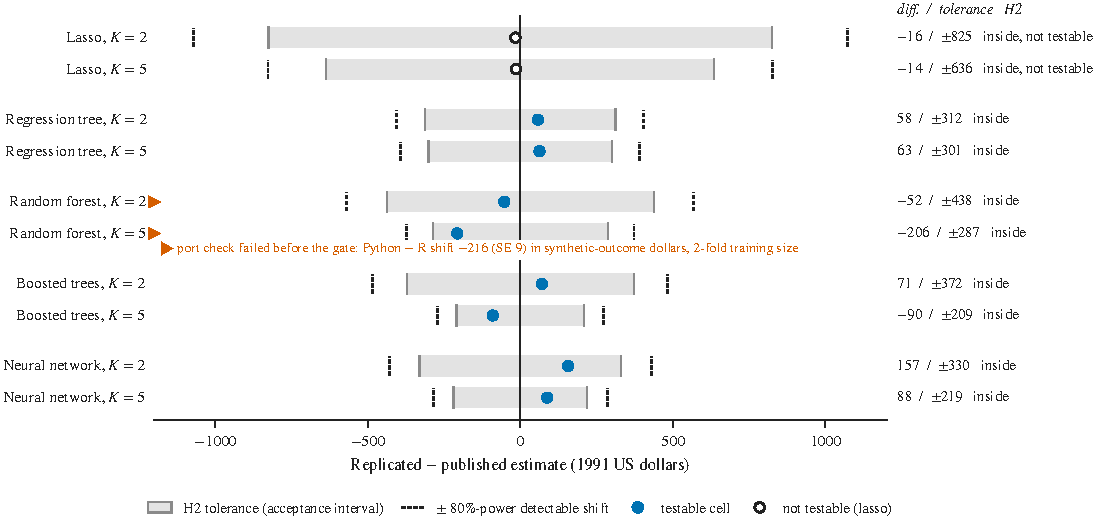
\includegraphics[width=\textwidth]{figures/fig_h2_diff.pdf}
\caption{Replicated minus published estimate for each cell, against the H2 acceptance
interval (1991 US dollars). Filled dots are testable cells; open dots are the two lasso
cells, which are not testable at this resolution. The gray band is the pre-registered
tolerance $\pm 2.81\sqrt{\text{se}_{\text{rep}}^2 + \text{se}_{\text{pub}}^2}$, built from
the split-sampling standard errors of both medians; dashed ticks mark $\pm$MDS$_{80}$.
The right-hand column gives the difference, the tolerance and the H2 reading. Every cell
lies inside its band ($\HTwoNOutside$ of 10 outside); a dot inside the band means no shift
larger than MDS$_{80}$ was detected. Arrows mark the random-forest rows, whose port failed
the pre-analysis check with a shift of $\PortShiftForest$ (SE \PortShiftSeForest)
synthetic-outcome dollars at the 2-fold training size; that shift is printed, not plotted,
because it is not on the real-data scale.}
\label{fig:diff}
\end{figure}

\subsection{H1}

All ten replicated estimates are positive, and every 95\% interval excludes zero. The
lowest lower bound, $\tilde\theta - 1.96\,\hat\sigma_{\text{adj}}$, is \$$\CiLowLassoTwo$
(lasso, 2-fold); Table~\ref{tab:effect} lists all ten. H1 holds, as the literature led us
to expect.

\subsection{H2, cell by cell}

No cell lies outside its tolerance ($\HTwoNOutside$ of 10), and $\HTwoNTestableInside$ of
the $\HTwoNTestable$ testable cells lie inside. Under the decision rule fixed before the
analysis, \emph{H2 holds}. In every testable cell, no shift larger than the cell's
80\%-power detectable shift was detected. Measured in units of the published bracketed
SE, the differences are small (Table~\ref{tab:effect}); the largest in absolute value is
$\DiffPubSeForestFive$ (forest, 5-fold). Below we discuss the cells by learner, in
increasing order of the caveats they carry.

\paragraph{Regression tree, boosted trees, neural network.} These ports passed the
pre-analysis check, and their six cells pass H2. The tree differences are $+\$\DiffTreeTwo$
and $+\$\DiffTreeFive$ against tolerances of \$$\TolTreeTwo$ and \$$\TolTreeFive$, so
shifts above \$$\MdsTreeTwo$ and \$$\MdsTreeFive$ were not detected. The boosting
differences are $+\$\DiffBoostingTwo$ and \negusd{\DiffBoostingFive}
(tolerances \$$\TolBoostingTwo$ and \$$\TolBoostingFive$; MDS$_{80}$ \$$\MdsBoostingTwo$ and
\$$\MdsBoostingFive$). The neural-network differences are $+\$\DiffNnetTwo$ and
$+\$\DiffNnetFive$ (tolerances \$$\TolNnetTwo$ and \$$\TolNnetFive$; MDS$_{80}$
\$$\MdsNnetTwo$ and \$$\MdsNnetFive$). The 2-fold neural-network cell has the largest
difference of these six in dollars. The boosting cells rest on
only $S = 30$ splits, which the tolerances already account for.

\paragraph{Random forest: the port deviation.} Both forest cells pass: the differences are
\negusd{\DiffForestTwo} (tolerance \$$\TolForestTwo$, MDS$_{80}$ \$$\MdsForestTwo$) and
\negusd{\DiffForestFive} (tolerance \$$\TolForestFive$, MDS$_{80}$ \$$\MdsForestFive$).
These passes need the most qualification of the eight. The forest port failed the
pre-analysis check: on synthetic data its estimate was $\PortShiftForest$ (SE
\PortShiftSeForest) synthetic-outcome dollars from \var{randomForest}'s. The 5-fold
difference lies close to that measured shift, while the 2-fold difference does not show
it. The shift was measured at the 2-fold training size only, and on a synthetic outcome.
Both differences lie below the cells' detectable shifts, so neither forest cell can tell a
zero shift from a shift of the measured size. The forest passes therefore do not show
that our forest behaves like \var{randomForest} on these data. They show only that no
shift larger than \$$\MdsForestTwo$ (2-fold) or \$$\MdsForestFive$ (5-fold) was detected.
Before the analysis, the plan had named the 5-fold forest cell as the most likely H2
failure (probability 0.24). It came out inside its tolerance.

\paragraph{Lasso: not testable, and a spread discrepancy.} The lasso medians differ from
the published ones by \negusd{\DiffLassoTwo} and \negusd{\DiffLassoFive}, inside
tolerances of \$$\TolLassoTwo$ and \$$\TolLassoFive$. Because their detectable shifts
(\$$\MdsLassoTwo$, \$$\MdsLassoFive$) exceed half the published bracketed SE, the cells
are \emph{inside the tolerance, not testable at this resolution}, and are not counted
as passes. The small differences invite a stronger reading, which the split
distributions do not support. The published lasso adjusted SEs are not matched. Our
adjusted SEs are $\SeAdjLassoTwo$ against $\PubSeAdjLassoTwo$ at $K = 2$ (ratio
$\SeAdjRatioLassoTwo$) and $\SeAdjLassoFive$ against $\PubSeAdjLassoFive$ at $K = 5$
(ratio $\SeAdjRatioLassoFive$), while the bracketed SEs agree closely ($\SeMedLassoTwo$
versus $\PubSeMedLassoTwo$; $\SeMedLassoFive$ versus $\PubSeMedLassoFive$). The gap comes
from the split-to-split spread. Our $1.4826 \times \text{MAD}$ of the split estimates is
\$$\SplitSdObsLassoTwo$ at $K = 2$ and \$$\SplitSdObsLassoFive$ at $K = 5$. The published
standard errors imply \$$\SplitSdPubLassoTwo$ and \$$\SplitSdPubLassoFive$, several
times more. For the other learners our spread is also narrower than the published one,
but by much less (Figure~\ref{fig:spread}). Of all the replicated estimates and standard
errors, these two lasso adjusted SEs are the only ones that miss the published values by
more than 15\%. No run tests why our lasso varies so much less across splits. A lasso
median that matches the published one closely while its split distribution is several
times narrower is weak evidence that our port behaves like the authors' lasso on
\var{net\_tfa}. We read the lasso cells only as ``inside, not testable''.

\subsection{H3}

At both fold counts the lasso estimate is below every flexible learner's estimate, so
H3 holds. The smallest margin, the lowest flexible-learner estimate minus the lasso
estimate, is \$$\HThreeMarginTwo$ at $K = 2$ and \$$\HThreeMarginFive$ at $K = 5$. In
both cases the closest flexible learner is the regression tree.

\subsection{Magnitudes}

Table~\ref{tab:effect} expresses each cell relative to the baseline. The replicated
estimates range from $\PctIneligLassoTwo$\% (lasso, 2-fold) to $\PctIneligNnetFive$\%
(neural network, 5-fold) of mean net financial assets among ineligible households
(\$$\BaselineInelig$), or $\SdUnitsLassoTwo$ to $\SdUnitsNnetFive$ standard deviations of
net financial assets; the published cells give nearly the same figures. Under the
identifying assumption these are weighted averages of conditional effects of eligibility,
not average treatment effects.

\begin{table}[t]
\centering
\caption{Effect sizes and H1. Replicated estimate; lower bound of its 95\% interval
($\tilde\theta - 1.96 \times$ adjusted SE); replicated and published estimate as a
percentage of mean net financial assets of ineligible households (\$$\BaselineInelig$)
and in standard deviations of net financial assets (\$$\BaselineSd$); and the replicated
minus published difference in units of the published bracketed SE. 1991 US dollars.}
\label{tab:effect}
{\footnotesize
\begin{tabular}{@{}l c r r rr rr r@{}}
\toprule
 & & & & \multicolumn{2}{c}{\% of ineligible mean} & \multicolumn{2}{c}{SD units} & Difference in \\
\cmidrule(lr){5-6}\cmidrule(lr){7-8}
Learner & $K$ & Estimate & 95\% lower bound & Repl. & Publ. & Repl. & Publ. & publ.\ bracketed SEs \\
\midrule
Lasso & 2 & $\ThetaLassoTwo$ & $\CiLowLassoTwo$ & $\PctIneligLassoTwo$ & $\PubPctIneligLassoTwo$ & $\SdUnitsLassoTwo$ & $\PubSdUnitsLassoTwo$ & $\DiffPubSeLassoTwo$ \\
 & 5 & $\ThetaLassoFive$ & $\CiLowLassoFive$ & $\PctIneligLassoFive$ & $\PubPctIneligLassoFive$ & $\SdUnitsLassoFive$ & $\PubSdUnitsLassoFive$ & $\DiffPubSeLassoFive$ \\
\addlinespace
Regression tree & 2 & $\ThetaTreeTwo$ & $\CiLowTreeTwo$ & $\PctIneligTreeTwo$ & $\PubPctIneligTreeTwo$ & $\SdUnitsTreeTwo$ & $\PubSdUnitsTreeTwo$ & $+\DiffPubSeTreeTwo$ \\
 & 5 & $\ThetaTreeFive$ & $\CiLowTreeFive$ & $\PctIneligTreeFive$ & $\PubPctIneligTreeFive$ & $\SdUnitsTreeFive$ & $\PubSdUnitsTreeFive$ & $+\DiffPubSeTreeFive$ \\
\addlinespace
Random forest & 2 & $\ThetaForestTwo$ & $\CiLowForestTwo$ & $\PctIneligForestTwo$ & $\PubPctIneligForestTwo$ & $\SdUnitsForestTwo$ & $\PubSdUnitsForestTwo$ & $\DiffPubSeForestTwo$ \\
 & 5 & $\ThetaForestFive$ & $\CiLowForestFive$ & $\PctIneligForestFive$ & $\PubPctIneligForestFive$ & $\SdUnitsForestFive$ & $\PubSdUnitsForestFive$ & $\DiffPubSeForestFive$ \\
\addlinespace
Boosted trees & 2 & $\ThetaBoostingTwo$ & $\CiLowBoostingTwo$ & $\PctIneligBoostingTwo$ & $\PubPctIneligBoostingTwo$ & $\SdUnitsBoostingTwo$ & $\PubSdUnitsBoostingTwo$ & $+\DiffPubSeBoostingTwo$ \\
 & 5 & $\ThetaBoostingFive$ & $\CiLowBoostingFive$ & $\PctIneligBoostingFive$ & $\PubPctIneligBoostingFive$ & $\SdUnitsBoostingFive$ & $\PubSdUnitsBoostingFive$ & $\DiffPubSeBoostingFive$ \\
\addlinespace
Neural network & 2 & $\ThetaNnetTwo$ & $\CiLowNnetTwo$ & $\PctIneligNnetTwo$ & $\PubPctIneligNnetTwo$ & $\SdUnitsNnetTwo$ & $\PubSdUnitsNnetTwo$ & $+\DiffPubSeNnetTwo$ \\
 & 5 & $\ThetaNnetFive$ & $\CiLowNnetFive$ & $\PctIneligNnetFive$ & $\PubPctIneligNnetFive$ & $\SdUnitsNnetFive$ & $\PubSdUnitsNnetFive$ & $+\DiffPubSeNnetFive$ \\
\bottomrule
\end{tabular}}
\end{table}

\subsection{Sensitivity: the lasso penalty constant}
\label{sec:sens}

The sensitivity run repeats the lasso with $c = 1.1$ for the outcome lasso, with
everything else unchanged. It is descriptive only; it supplies no cell value and changes
no verdict. With $c = 1.1$ the lasso estimates are \$$\SensCElevenThetaTwo$ (adjusted SE
$\SensCElevenSeAdjTwo$) at $K = 2$ and \$$\SensCElevenThetaFive$ (adjusted SE
$\SensCElevenSeAdjFive$) at $K = 5$. These are \negusd{\SensCElevenMinusMainTwo} and
\negusd{\SensCElevenMinusMainFive} relative to the primary $c = 0.5$ lasso, and
\negusd{\SensCElevenDiffTwo} and \negusd{\SensCElevenDiffFive} relative to the published
cells. Both lie inside the lasso tolerances, and the H3 ordering also holds with them
(margins \$$\SensCElevenHThreeMarginTwo$ and \$$\SensCElevenHThreeMarginFive$).

The primary lasso lies closer to the published cells than the $c = 1.1$ run. Both lie
inside tolerances that cannot test the lasso cells, so the data do not show which
\var{hdm} version the authors ran. That the authors' outcome lasso used $c = 0.5$ is a
\emph{conjecture}. It rests on the version timeline, not on our estimates. The published
Table~2 numbers first appear in the arXiv version of 21 June 2017, after a version of 30
December 2016 that reports an earlier run \citep{chernozhukov2018dml}. Throughout that
window the CRAN release of \var{hdm} was 0.2.0, which applies $c = 0.5$. Version 0.2.3,
the only one that keeps $c = 1.1$, was released on 23 January 2018 \citep{hdm_cran}. An
unreleased development build or a stale 0.1.0 installation (effective $c$ of about 0.62)
cannot be excluded.

% ---------------------------------------------------------------------------------------
\section{Diagnostics}
\label{sec:diagnostics}

The diagnostics below were planned in the design. None of them changes a tolerance, the
number of splits, a claim or a verdict.

\begin{figure}[t]
\centering
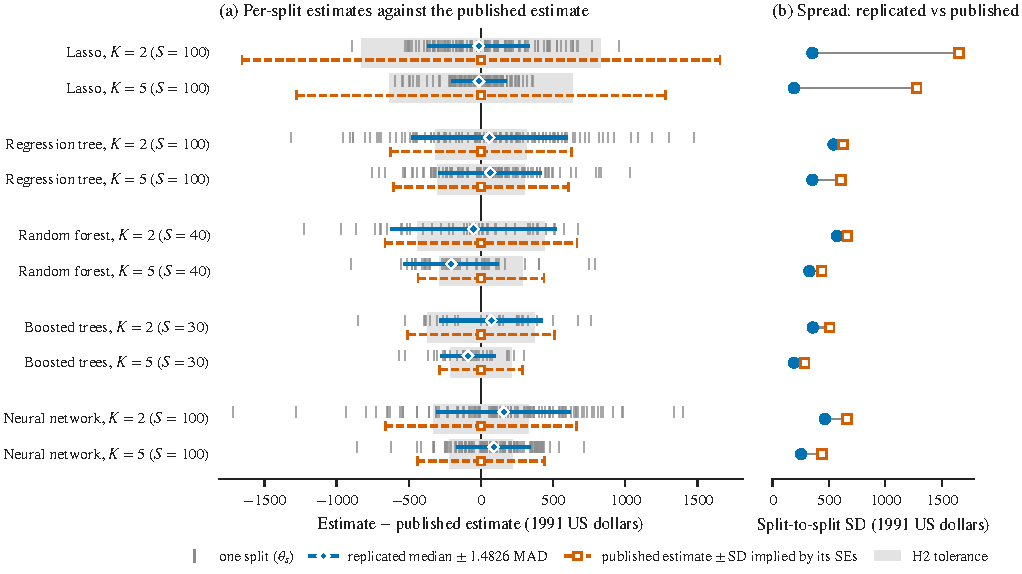
\includegraphics[width=\textwidth]{figures/fig_split_spread.pdf}
\caption{Split-to-split spread of the replicated estimates against the spread implied by
the published SEs (1991 US dollars). Each row is one learner and fold count; $S$ is in
the row label. Panel~(a): every per-split estimate $\hat\theta_s$ minus the published
estimate (gray ticks). The blue diamond and solid bar show the replicated median
$\pm 1.4826 \times \text{MAD}$ of the $\hat\theta_s$; the vermillion square and dashed
bar show the published estimate (zero on this axis) $\pm$ the split-to-split SD the
published SEs imply, $1.4826\,(\text{adj}^2 - \text{med}^2)^{1/2}$; the gray band is the
H2 tolerance. Panel~(b): the replicated spread (filled circle) and the published-implied
spread (open square) on an axis starting at zero. For every learner the replicated spread
is narrower; the lasso gap is by far the largest (\$$\SplitSdObsLassoTwo$ against
\$$\SplitSdPubLassoTwo$ at $K = 2$; \$$\SplitSdObsLassoFive$ against
\$$\SplitSdPubLassoFive$ at $K = 5$). No run tests why. The bars are spreads of the split
distribution, not confidence intervals for the median.}
\label{fig:spread}
\end{figure}

\paragraph{Split spread and standard errors.} Figure~\ref{fig:spread} and
Table~\ref{tab:diag} compare our split-to-split spread with the one the published SEs
imply. For every learner ours is narrower, and for the lasso by far the most. Our
bracketed SEs are within a few percent of the published ones in every cell. The ratios
range from $\SeMedRatioForestFive$ (forest, 5-fold) to $\SeMedRatioNnetFive$ (neural
network, 5-fold). The adjusted SEs agree as closely except for the two lasso cells
(Section~\ref{sec:results}). The descriptive tolerance computed from our own split
spread, $\text{tol}_{\text{obs}}$, is smaller than the pre-registered tolerance in every
cell, and every difference lies inside it as well.

\paragraph{Nuisance fit and overlap.} The median out-of-fold RMSE of $\hat\ell$ is between
\$$\RmseLBoostingFive$ (boosting, 5-fold) and \$$\RmseLTreeTwo$ (tree, 2-fold); that of
$\hat m$ is between $\RmseMBoostingFive$ and $\RmseMForestFive$. The random forest has the
highest $\hat m$ RMSE of the five learners at both fold counts. This is the direction the
port check found on synthetic data (a noisier Python treatment forest), but no run
compares our forest with \var{randomForest} on the real data. The share of out-of-fold
$\hat m$ outside $[0.01, 0.99]$ is zero for the lasso, tree and boosting. It is
$\MOutForestTwo$ and $\MOutForestFive$ for the forest and $\MOutNnetTwo$ and $\MOutNnetFive$
for the neural network (2- and 5-fold). No trimming is applied, as in the authors' PLR
code.

\paragraph{Neural-network convergence.} The median number of L-BFGS iterations is
$\NnetIterY$ for the outcome network and $\NnetIterD$, the iteration cap, for the
treatment network. The treatment network thus usually stops at the cap. In the port check
this also happened, and the Python and R treatment networks agreed with each other as
closely as two R seeds did.

\begin{table}[t]
\centering
\caption{Diagnostics (1991 US dollars except ratios and shares). Split SD: $1.4826 \times
\text{MAD}$ of our split estimates, and the value implied by the published SEs. Implied
MAD: $(\text{adj}^2 - \text{med}^2)^{1/2}$ for our aggregates and for the published ones.
SE ratios: replicated over published bracketed and adjusted SE. Tolerance and
$\text{tol}_{\text{obs}}$: the pre-registered H2 tolerance, and the descriptive one built
from our own split spread. RMSE: median over splits of the out-of-fold RMSE of $\hat\ell$
and $\hat m$. $\hat m$ out: median share of out-of-fold $\hat m$ outside $[0.01, 0.99]$.}
\label{tab:diag}
{\footnotesize\resizebox{\textwidth}{!}{%
\begin{tabular}{@{}l c rr rr rr rr rr r@{}}
\toprule
 & & \multicolumn{2}{c}{Split SD} & \multicolumn{2}{c}{Implied MAD} & \multicolumn{2}{c}{SE ratio} & & & \multicolumn{2}{c}{RMSE} & \\
\cmidrule(lr){3-4}\cmidrule(lr){5-6}\cmidrule(lr){7-8}\cmidrule(lr){11-12}
Learner & $K$ & Repl. & Publ. & Repl. & Publ. & Brack. & Adj. & Tolerance & $\text{tol}_{\text{obs}}$ & $\hat\ell$ & $\hat m$ & $\hat m$ out \\
\midrule
Lasso & 2 & $\SplitSdObsLassoTwo$ & $\SplitSdPubLassoTwo$ & $\ImpliedMadObsLassoTwo$ & $\ImpliedMadPubLassoTwo$ & $\SeMedRatioLassoTwo$ & $\SeAdjRatioLassoTwo$ & $\TolLassoTwo$ & $\TolObsLassoTwo$ & $\RmseLLassoTwo$ & $\RmseMLassoTwo$ & $\MOutLassoTwo$ \\
 & 5 & $\SplitSdObsLassoFive$ & $\SplitSdPubLassoFive$ & $\ImpliedMadObsLassoFive$ & $\ImpliedMadPubLassoFive$ & $\SeMedRatioLassoFive$ & $\SeAdjRatioLassoFive$ & $\TolLassoFive$ & $\TolObsLassoFive$ & $\RmseLLassoFive$ & $\RmseMLassoFive$ & $\MOutLassoFive$ \\
\addlinespace
Regression tree & 2 & $\SplitSdObsTreeTwo$ & $\SplitSdPubTreeTwo$ & $\ImpliedMadObsTreeTwo$ & $\ImpliedMadPubTreeTwo$ & $\SeMedRatioTreeTwo$ & $\SeAdjRatioTreeTwo$ & $\TolTreeTwo$ & $\TolObsTreeTwo$ & $\RmseLTreeTwo$ & $\RmseMTreeTwo$ & $\MOutTreeTwo$ \\
 & 5 & $\SplitSdObsTreeFive$ & $\SplitSdPubTreeFive$ & $\ImpliedMadObsTreeFive$ & $\ImpliedMadPubTreeFive$ & $\SeMedRatioTreeFive$ & $\SeAdjRatioTreeFive$ & $\TolTreeFive$ & $\TolObsTreeFive$ & $\RmseLTreeFive$ & $\RmseMTreeFive$ & $\MOutTreeFive$ \\
\addlinespace
Random forest & 2 & $\SplitSdObsForestTwo$ & $\SplitSdPubForestTwo$ & $\ImpliedMadObsForestTwo$ & $\ImpliedMadPubForestTwo$ & $\SeMedRatioForestTwo$ & $\SeAdjRatioForestTwo$ & $\TolForestTwo$ & $\TolObsForestTwo$ & $\RmseLForestTwo$ & $\RmseMForestTwo$ & $\MOutForestTwo$ \\
 & 5 & $\SplitSdObsForestFive$ & $\SplitSdPubForestFive$ & $\ImpliedMadObsForestFive$ & $\ImpliedMadPubForestFive$ & $\SeMedRatioForestFive$ & $\SeAdjRatioForestFive$ & $\TolForestFive$ & $\TolObsForestFive$ & $\RmseLForestFive$ & $\RmseMForestFive$ & $\MOutForestFive$ \\
\addlinespace
Boosted trees & 2 & $\SplitSdObsBoostingTwo$ & $\SplitSdPubBoostingTwo$ & $\ImpliedMadObsBoostingTwo$ & $\ImpliedMadPubBoostingTwo$ & $\SeMedRatioBoostingTwo$ & $\SeAdjRatioBoostingTwo$ & $\TolBoostingTwo$ & $\TolObsBoostingTwo$ & $\RmseLBoostingTwo$ & $\RmseMBoostingTwo$ & $\MOutBoostingTwo$ \\
 & 5 & $\SplitSdObsBoostingFive$ & $\SplitSdPubBoostingFive$ & $\ImpliedMadObsBoostingFive$ & $\ImpliedMadPubBoostingFive$ & $\SeMedRatioBoostingFive$ & $\SeAdjRatioBoostingFive$ & $\TolBoostingFive$ & $\TolObsBoostingFive$ & $\RmseLBoostingFive$ & $\RmseMBoostingFive$ & $\MOutBoostingFive$ \\
\addlinespace
Neural network & 2 & $\SplitSdObsNnetTwo$ & $\SplitSdPubNnetTwo$ & $\ImpliedMadObsNnetTwo$ & $\ImpliedMadPubNnetTwo$ & $\SeMedRatioNnetTwo$ & $\SeAdjRatioNnetTwo$ & $\TolNnetTwo$ & $\TolObsNnetTwo$ & $\RmseLNnetTwo$ & $\RmseMNnetTwo$ & $\MOutNnetTwo$ \\
 & 5 & $\SplitSdObsNnetFive$ & $\SplitSdPubNnetFive$ & $\ImpliedMadObsNnetFive$ & $\ImpliedMadPubNnetFive$ & $\SeMedRatioNnetFive$ & $\SeAdjRatioNnetFive$ & $\TolNnetFive$ & $\TolObsNnetFive$ & $\RmseLNnetFive$ & $\RmseMNnetFive$ & $\MOutNnetFive$ \\
\bottomrule
\end{tabular}}}
\end{table}

\paragraph{Wall time.} The design estimated 34--43 minutes of wall time for the main
analysis and warned that 70--100 minutes was possible. The analysis runs took 92 minutes
in all (runs/NOTES.md), against a 60-minute budget. The machine was shared with other
heavy jobs during the outcome-lasso run: the load average was 46--90 on 8 cores, and the
lasso main run took 52 minutes, while the $c = 1.1$ lasso run, with the same code under
lighter load, took 11. Under the rule fixed at the design gate, the overrun is disclosed
and was not traded for power: no number of splits was changed and no run was cut short.
Every fit is seeded, so the load affects time only, not the numbers.

\FloatBarrier
% ---------------------------------------------------------------------------------------
\section{Limitations}
\label{sec:limitations}

\paragraph{Power.} A pass rules out only shifts larger than the cell's detectable shift,
\$$\MdsBoostingFive$ to \$$\MdsForestTwo$ on the testable cells. Implementations that
differ from the authors' by a few hundred dollars can pass. The two lasso cells, the most
implementation-sensitive, cannot be confirmed at any affordable number of splits. The
small $S$ for the forest (40) and boosting (30) widens their tolerances.

\paragraph{The port check is narrow.} It used a synthetic outcome on a smaller scale than
\var{net\_tfa}, only the 2-fold training size and ten units. A port that passes it can
still differ on the real data, and the \$25 floors in its pass rules are in synthetic
dollars, not real-data tolerances. The 5-fold readings assume that the 2-fold
deviations carry over.

\paragraph{Unexplained differences.} The forest port's deviation and the narrow lasso
split spread are both unexplained. The split-search explanation for the forest is a
conjecture, and no run tests the cause of the lasso spread. With one re-implementation
we cannot separate software from tuning differences, and the authors' package versions
are unknown.

\paragraph{Tolerance assumptions.} The tolerances assume roughly normal split noise; the
factor 1.4826 is an upper bound when within-split variance differs across splits, which
makes them conservative. The familywise rate treats the ten cells as independent,
although learners share splits within a fold count.

\paragraph{Identification and inference.} The PLR coefficient is causal only under
conditional exogeneity of eligibility, which this study does not test, and it is not the
average treatment effect. Standard errors are HC0 at the household level, as published.
Eligibility varies by employer, but the file has no employer identifier, so clustering is
impossible. This does not affect point estimates or H2.

\paragraph{Scope.} We do not replicate the Ensemble and Best columns, Panel~A or the
participation estimates. The novelty claim rests on the literature and documentation we
read, not on a systematic search of code repositories.

\paragraph{Replication.} All runs were made on one machine. The lasso and neural-network
fits use BLAS-dependent floating point, so a rerun on another machine may differ beyond
the protocol's tolerance. The clean rerun required before release is pending (AI-use
statement).

% ---------------------------------------------------------------------------------------
\section{Deviations and disclosures}
\label{sec:deviations}

\paragraph{Deviations in the analysis runs.} There were none. Every analysis run used
the command, number of splits and specification written before the design gate, in the
planned order, and every run exited without error (runs/NOTES.md). Two events are
disclosed:
\begin{enumerate}
  \item \emph{Budget overrun.} The runs took 92 minutes against the 60-minute budget
        (Section~\ref{sec:diagnostics}). Under the design's rule the overrun is disclosed,
        and $S$ was not reduced.
  \item \emph{Run restart.} The first attempt at the outcome-lasso main run was interrupted
        by a restart of the Econometrician's session. It had written an incomplete run
        record, which was removed before the new session was launched; nothing from it was
        read, kept or reported. The lasso main run was then repeated from scratch with the
        same command and seeds, so the restart changes no number. The relaunch brief is
        archived in the workspace.
\end{enumerate}

\paragraph{Amendments to H2 after the question gate.} Both were made at the design stage,
before the design gate and before any analysis run. The human saw them at the design
gate.
\begin{enumerate}
  \item At the Reviewer's request (design review round~1, finding F1), the
        ``not testable'' rule was made one-sided. Originally a not-testable cell did not
        count either way. Now a not-testable cell outside its tolerance fails H2. This makes
        H2 stricter.
  \item At the PI's request (design review round~2, finding F7), the sentence of H2 that
        states its false-failure rate was amended. It now gives the rate under the port
        deviations measured before the gate (about 33\% after the lasso correction, with
        the forest deviation remaining) instead of 5\%. A fixed reading rule for failed
        cells was added at the same time.
\end{enumerate}

\paragraph{Other changes before any analysis run.}
\begin{itemize}
  \item The lasso port gained \var{hdm}'s zero threshold after the code review, by the
        PI's ruling. The design was amended to say so and the port check was re-run; the
        first check's result is kept in the run notes (Section~\ref{sec:impl}).
  \item The forest port was kept as specified after it failed the port check, by the
        PI's ruling. Its deviation was priced into H2 rather than removed by re-tuning.
  \item The numbers of splits were kept after the port check's timing suggested a 70--100
        minute analysis, by the PI's ruling. Any overrun was to be disclosed rather than
        traded for power.
\end{itemize}

\paragraph{Departures from the authors' protocol, built into the design.} We use
Python and scikit-learn instead of R, with different random partitions and seeds. We use
fewer splits for the forest (40) and boosting (30). We do not estimate the Ensemble and
Best columns. Our outcome lasso uses an assumed penalty constant (Section~\ref{sec:impl}).

\paragraph{Other disclosures.}
\begin{itemize}
  \item During the first review of the research question, the Reviewer timed a single
        random-forest fit and a single boosting fit to check feasibility. No estimate of
        the eligibility coefficient was computed.
  \item Several checks during the work were made outside the logged runs (smoke tests of
        the code on synthetic data, and some of the Reviewer's diagnostics). They are
        labelled as unlogged in the run notes and reviews, and no number in this paper
        comes from them.
  \item After the first two results reviews, the text of some claims was reworded (the
        meaning of a pass, the forest caveats, the lasso spread, the units of the port
        shifts). No run, code or plan value changed.
\end{itemize}

% ---------------------------------------------------------------------------------------
\section{Conclusion}
\label{sec:conclusion}

An implementation of the published double machine learning procedure written without the
authors' code, with scikit-learn ports of their learners, gives ten PLR estimates of the
401(k) eligibility coefficient that all lie within the pre-registered split-noise
tolerances of \citet[Table~2, Panel~B]{chernozhukov2018dml}. H2 holds in the sense fixed
before the analysis. In each of the eight testable cells, no shift larger than the
cell's 80\%-power detectable shift, at most \$$\MdsForestTwo$, was detected; smaller
shifts remain possible. The forest passes coexist with a forest port that failed its
check against R. The lasso cells cannot be tested at this resolution, and their narrow
split spread leaves the published lasso adjusted SEs unmatched. The results confirm, as
expected, that every estimate is positive and significant and that the lasso gives the
smallest estimate. For readers who use this application as a benchmark, the main lessons
concern precision, not the sign or size of the effect. Even with 100 splits, a
cell-by-cell check of these estimates cannot see shifts of a few hundred dollars. The
treatment forest and the lasso's split-to-split variability are where an independent
implementation is most likely to depart from the original.

\section*{AI-use statement}

This paper was drafted by a crew of AI research-assistant agents
(Free-Research-Crew, protocol v0.1) under the direction of the human author, Bryce Wang.
He approved the research question (2026-11-18, 12:24 UTC), the design (2026-11-18,
14:38 UTC) and the results (2026-11-19, 06:57 UTC) at three human gates, each in chat
after reading the Reviewer's verdict. The manuscript itself is subject to a fourth, the
submission gate. He takes responsibility for the paper's content.

\begin{itemize}
  \item \textbf{Roles and models.} Every crew role ran on Anthropic Claude through Claude
        Code. The PI role was the main Claude Code session. The Scout, Data RA, Designer,
        Econometrician, Figures RA, Reviewer and Writer ran as subagents launched from
        that session; the Replicator has not yet run. The review records name the model as
        \texttt{claude-opus-5-5}. The Econometrician's session was restarted once during
        the analysis runs (Section~\ref{sec:deviations}). Briefs to the agents were archived
        in \texttt{briefs/} from the Econometrician's relaunch brief (2026-11-18, 16:09 UTC)
        onward. Earlier briefs were not archived.
  \item \textbf{Review.} The Reviewer agent ran 4 rounds on the research question, 3 on the
        design, 2 on the code and 2 on the results. No separate literature round was held,
        and no review of the paper has been held yet. The code was reviewed, and passed,
        before any analysis run. Its independence level was \emph{fresh-context}: a new
        context in every round, with the same model family as the other roles. The human
        author chose this over a cross-family reviewer. Three final rounds passed with
        minor findings still open:
        \begin{itemize}
          \item question round~4 (three findings), carried to the design stage and resolved
                there;
          \item design round~3 (two findings), answered in the plan before the design gate;
          \item results round~2 (one finding), answered in the claims before the results
                gate.
        \end{itemize}
  \item \textbf{Findings accepted over the Reviewer's objection.} None.
  \item \textbf{Evidence.} Every result number in the text and tables is a macro generated
        from the metrics of a logged run, or is written by a logged table script from run
        metrics. The numbers typed by hand are of three kinds:
        \begin{itemize}
          \item design facts fixed in the plan before any analysis run, including the
                tolerance constants, the numbers of splits, the timing estimates, the
                half-SE thresholds, the per-cell false-failure probabilities and the
                combined 33\% rate;
          \item published or source facts, quoted as the Scout's source notes record them;
          \item process facts: dates, review-round counts, and the 92-minute wall time
                with its load figures, taken from \texttt{runs/NOTES.md} and the run
                records.
        \end{itemize}
        Every citation was checked against its source by the Scout: 17 from the full text,
        2 from the abstract only and 1 by resolving its DOI. Where only the abstract or
        metadata could be read (as for \citet{chernozhukov2004}, \citet{poterba1995} and
        \citet{abadie2003}), the paper cites the source for no more than that. The full
        workspace is public at
        \url{https://github.com/brycewang-stanford/Free-Research-Crew/tree/main/gallery/ss-dml-401k}.
        It contains the plan, the run ledger and notes, the code (with a verbatim copy of
        the authors' \texttt{ML\_Functions.R}), the data manifest, every review, the
        archived briefs and the source notes.
  \item \textbf{Replication.} Pending. No \texttt{replication.json} exists at the time of
        writing. The Replicator's clean rerun from \texttt{code/requirements.txt} is
        required before the submission gate, and its result will be reported here.
\end{itemize}


\bibliographystyle{plainnat}
\bibliography{../refs}

\end{document}
